% Options for packages loaded elsewhere
\PassOptionsToPackage{unicode}{hyperref}
\PassOptionsToPackage{hyphens}{url}
%
\documentclass[
  man,floatsintext]{apa6}
\usepackage{amsmath,amssymb}
\usepackage{lmodern}
\usepackage{iftex}
\ifPDFTeX
  \usepackage[T1]{fontenc}
  \usepackage[utf8]{inputenc}
  \usepackage{textcomp} % provide euro and other symbols
\else % if luatex or xetex
  \usepackage{unicode-math}
  \defaultfontfeatures{Scale=MatchLowercase}
  \defaultfontfeatures[\rmfamily]{Ligatures=TeX,Scale=1}
\fi
% Use upquote if available, for straight quotes in verbatim environments
\IfFileExists{upquote.sty}{\usepackage{upquote}}{}
\IfFileExists{microtype.sty}{% use microtype if available
  \usepackage[]{microtype}
  \UseMicrotypeSet[protrusion]{basicmath} % disable protrusion for tt fonts
}{}
\makeatletter
\@ifundefined{KOMAClassName}{% if non-KOMA class
  \IfFileExists{parskip.sty}{%
    \usepackage{parskip}
  }{% else
    \setlength{\parindent}{0pt}
    \setlength{\parskip}{6pt plus 2pt minus 1pt}}
}{% if KOMA class
  \KOMAoptions{parskip=half}}
\makeatother
\usepackage{xcolor}
\usepackage{graphicx}
\makeatletter
\def\maxwidth{\ifdim\Gin@nat@width>\linewidth\linewidth\else\Gin@nat@width\fi}
\def\maxheight{\ifdim\Gin@nat@height>\textheight\textheight\else\Gin@nat@height\fi}
\makeatother
% Scale images if necessary, so that they will not overflow the page
% margins by default, and it is still possible to overwrite the defaults
% using explicit options in \includegraphics[width, height, ...]{}
\setkeys{Gin}{width=\maxwidth,height=\maxheight,keepaspectratio}
% Set default figure placement to htbp
\makeatletter
\def\fps@figure{htbp}
\makeatother
\setlength{\emergencystretch}{3em} % prevent overfull lines
\providecommand{\tightlist}{%
  \setlength{\itemsep}{0pt}\setlength{\parskip}{0pt}}
\setcounter{secnumdepth}{-\maxdimen} % remove section numbering
% Make \paragraph and \subparagraph free-standing
\ifx\paragraph\undefined\else
  \let\oldparagraph\paragraph
  \renewcommand{\paragraph}[1]{\oldparagraph{#1}\mbox{}}
\fi
\ifx\subparagraph\undefined\else
  \let\oldsubparagraph\subparagraph
  \renewcommand{\subparagraph}[1]{\oldsubparagraph{#1}\mbox{}}
\fi
\newlength{\cslhangindent}
\setlength{\cslhangindent}{1.5em}
\newlength{\csllabelwidth}
\setlength{\csllabelwidth}{3em}
\newlength{\cslentryspacingunit} % times entry-spacing
\setlength{\cslentryspacingunit}{\parskip}
\newenvironment{CSLReferences}[2] % #1 hanging-ident, #2 entry spacing
 {% don't indent paragraphs
  \setlength{\parindent}{0pt}
  % turn on hanging indent if param 1 is 1
  \ifodd #1
  \let\oldpar\par
  \def\par{\hangindent=\cslhangindent\oldpar}
  \fi
  % set entry spacing
  \setlength{\parskip}{#2\cslentryspacingunit}
 }%
 {}
\usepackage{calc}
\newcommand{\CSLBlock}[1]{#1\hfill\break}
\newcommand{\CSLLeftMargin}[1]{\parbox[t]{\csllabelwidth}{#1}}
\newcommand{\CSLRightInline}[1]{\parbox[t]{\linewidth - \csllabelwidth}{#1}\break}
\newcommand{\CSLIndent}[1]{\hspace{\cslhangindent}#1}
\ifLuaTeX
\usepackage[bidi=basic]{babel}
\else
\usepackage[bidi=default]{babel}
\fi
\babelprovide[main,import]{english}
% get rid of language-specific shorthands (see #6817):
\let\LanguageShortHands\languageshorthands
\def\languageshorthands#1{}
% Manuscript styling
\usepackage{upgreek}
\captionsetup{font=singlespacing,justification=justified}

% Table formatting
\usepackage{longtable}
\usepackage{lscape}
% \usepackage[counterclockwise]{rotating}   % Landscape page setup for large tables
\usepackage{multirow}		% Table styling
\usepackage{tabularx}		% Control Column width
\usepackage[flushleft]{threeparttable}	% Allows for three part tables with a specified notes section
\usepackage{threeparttablex}            % Lets threeparttable work with longtable

% Create new environments so endfloat can handle them
% \newenvironment{ltable}
%   {\begin{landscape}\centering\begin{threeparttable}}
%   {\end{threeparttable}\end{landscape}}
\newenvironment{lltable}{\begin{landscape}\centering\begin{ThreePartTable}}{\end{ThreePartTable}\end{landscape}}

% Enables adjusting longtable caption width to table width
% Solution found at http://golatex.de/longtable-mit-caption-so-breit-wie-die-tabelle-t15767.html
\makeatletter
\newcommand\LastLTentrywidth{1em}
\newlength\longtablewidth
\setlength{\longtablewidth}{1in}
\newcommand{\getlongtablewidth}{\begingroup \ifcsname LT@\roman{LT@tables}\endcsname \global\longtablewidth=0pt \renewcommand{\LT@entry}[2]{\global\advance\longtablewidth by ##2\relax\gdef\LastLTentrywidth{##2}}\@nameuse{LT@\roman{LT@tables}} \fi \endgroup}

% \setlength{\parindent}{0.5in}
% \setlength{\parskip}{0pt plus 0pt minus 0pt}

% Overwrite redefinition of paragraph and subparagraph by the default LaTeX template
% See https://github.com/crsh/papaja/issues/292
\makeatletter
\renewcommand{\paragraph}{\@startsection{paragraph}{4}{\parindent}%
  {0\baselineskip \@plus 0.2ex \@minus 0.2ex}%
  {-1em}%
  {\normalfont\normalsize\bfseries\itshape\typesectitle}}

\renewcommand{\subparagraph}[1]{\@startsection{subparagraph}{5}{1em}%
  {0\baselineskip \@plus 0.2ex \@minus 0.2ex}%
  {-\z@\relax}%
  {\normalfont\normalsize\itshape\hspace{\parindent}{#1}\textit{\addperi}}{\relax}}
\makeatother

% \usepackage{etoolbox}
\makeatletter
\patchcmd{\HyOrg@maketitle}
  {\section{\normalfont\normalsize\abstractname}}
  {\section*{\normalfont\normalsize\abstractname}}
  {}{\typeout{Failed to patch abstract.}}
\patchcmd{\HyOrg@maketitle}
  {\section{\protect\normalfont{\@title}}}
  {\section*{\protect\normalfont{\@title}}}
  {}{\typeout{Failed to patch title.}}
\makeatother

\usepackage{xpatch}
\makeatletter
\xapptocmd\appendix
  {\xapptocmd\section
    {\addcontentsline{toc}{section}{\appendixname\ifoneappendix\else~\theappendix\fi\\: #1}}
    {}{\InnerPatchFailed}%
  }
{}{\PatchFailed}
\keywords{keywords\newline\indent Word count: X}
\usepackage{lineno}

\linenumbers
\usepackage{csquotes}
\usepackage{float}
\ifLuaTeX
  \usepackage{selnolig}  % disable illegal ligatures
\fi
\IfFileExists{bookmark.sty}{\usepackage{bookmark}}{\usepackage{hyperref}}
\IfFileExists{xurl.sty}{\usepackage{xurl}}{} % add URL line breaks if available
\urlstyle{same} % disable monospaced font for URLs
\hypersetup{
  pdftitle={Supplementary Materials: Cognitive Load and Moral Dumbfounding},
  pdfauthor={Cillian McHugh1, Marek McGann2, Eric R. Igou1, \& Elaine L. Kinsella1},
  pdflang={en-EN},
  pdfkeywords={keywords},
  hidelinks,
  pdfcreator={LaTeX via pandoc}}

\title{Supplementary Materials: Cognitive Load and Moral Dumbfounding}
\author{Cillian McHugh\textsuperscript{1}, Marek McGann\textsuperscript{2}, Eric R. Igou\textsuperscript{1}, \& Elaine L. Kinsella\textsuperscript{1}}
\date{}


\shorttitle{Cognitive Load and Moral Dumbfounding}

\authornote{

Correspondence concerning this article should be addressed to Cillian McHugh, Department of Psychology, University of Limerick. E-mail: \href{mailto:cillian.mchugh@ul.ie}{\nolinkurl{cillian.mchugh@ul.ie}}

}

\affiliation{\vspace{0.5cm}\textsuperscript{1} Department of Psychology, University of Limerick\\\textsuperscript{2} Department of Psychology, Mary Immaculate College, University of Limerick}

\begin{document}
\maketitle

\hypertarget{supplementary-materials}{%
\section{Supplementary Materials}\label{supplementary-materials}}

\hypertarget{scenarios}{%
\subsection{Scenarios}\label{scenarios}}

\hypertarget{julie-and-mark}{%
\subsubsection{Julie and Mark}\label{julie-and-mark}}

Julie and Mark, who are brother and sister are travelling together in France. They are both on summer vacation from college. One night they are staying alone in a cabin near the beach. They decide that it would be interesting and fun if they tried making love. At very least it would be a new experience for each of them. Julie was already taking birth control pills, but Mark uses a condom too, just to be safe. They both enjoy it, but they decide not to do it again. They keep that night as a special secret between them, which makes them feel even closer to each other.

\hypertarget{jennifer}{%
\subsubsection{Jennifer}\label{jennifer}}

Jennifer works in a medical school pathology lab as a research assistant. The lab prepares human cadavers that are used to teach medical students about anatomy. The cadavers come from people who had donated their body to science for research. One night Jennifer is leaving the lab when she sees a body that is going to be discarded the next day. Jennifer was a vegetarian, for moral reasons. She thought it was wrong to kill animals for food. But then, when she saw a body about to be cremated, she thought it was irrational to waste perfectly edible meat. So she cut off a piece of flesh, and took it home and cooked it. The person had died recently of a heart attack, and she cooked the meat thoroughly, so there was no risk of disease.

\hypertarget{trolley}{%
\subsubsection{Trolley}\label{trolley}}

A Trolley is hurtling down a track towards five people. It will kill them all on impact. Paul is on a bridge under which it will pass. He can stop it by putting something very heavy in front of it. As it happens, there is a very fat man next to him. Paul's only way to stop the trolley is to push him over the bridge and onto the track, killing him to save five. Paul decides to push the man.

\hypertarget{heinz}{%
\subsubsection{Heinz}\label{heinz}}

In Europe, a woman was near death from a very bad disease, a special kind of cancer. There was one drug that the doctors thought might save her. It was a form of radium for which a Druggist was charging ten times what the drug cost him to make. The sick woman's husband, Heinz, went to everyone he knew to borrow the money, but he could only get together about half of what it cost. He told the Druggist that his wife was dying, and asked him to sell it cheaper or let him pay later. But the Druggist said, `No, I discovered the drug and I'm going to make money from it.' So, Heinz got desperate and broke into the man's store to steal the drug for his wife. The Druggist had Heinz arrested and charge.

\hypertarget{measures}{%
\subsection{Measures}\label{measures}}

\hypertarget{julie-and-mark-1}{%
\subsubsection{Julie and Mark}\label{julie-and-mark-1}}

\begin{itemize}
\tightlist
\item
  How would you rate the behaviour of Julie and Mark? (1 = Morally Wrong; and 7 = Morally Right)
\item
  How confident are you about your judgement? (1 = Not at all Confident; 7 = Extremely Confident)
\item
  Do you agree that any concerns regarding reproductive complications are eased by their using of two forms of contraception? (Yes/No)
\item
  And do you accept that they are both consenting adults, and that they both consented and enjoyed it? (Yes/No)
\item
  And do you concede that nobody else was affected by their actions? (Yes/No)
\item
  Julie and Mark's behaviour did not harm anyone or negatively affect anyone. How can there be anything wrong with what they did?
\end{itemize}

\hypertarget{jennifer-1}{%
\subsubsection{Jennifer}\label{jennifer-1}}

\begin{itemize}
\tightlist
\item
  How would you rate the behaviour of Jennifer? (1 = Morally Wrong; 7 = Morally Right)
\item
  How confident are you about your judgement? (1 = Not at all Confident; 7 = Extremely Confident)
\item
  The body had been donated for research, it was to be discarded the next day. You must agree then that it had obviously fulfilled its purpose?
\item
  Do you accept that the body was already dead?
\item
  And do you accept that there was no risk of disease?
\item
  Jennifer's actions did not harm anyone, or negatively affect anyone. How can there be anything wrong with what she did?
\end{itemize}

\hypertarget{trolley-1}{%
\subsubsection{Trolley}\label{trolley-1}}

\begin{itemize}
\tightlist
\item
  How would you rate the actions of Paul? (1 = Morally Wrong; and 7 = Morally Right)
\item
  How confident are you about your judgement? (1 = Not at all Confident; 7 = Extremely Confident)
\item
  Do you accept that five people would have died if Paul didn't push the man?
\item
  And this man is the only way available to stop the trolley? (Paul does not weigh enough)
\item
  Do you agree that in stopping the trolley Paul saved the lives of five people?
\item
  Paul's actions saved the lives of five people! How can saving lives be wrong?
\end{itemize}

\hypertarget{heinz-1}{%
\subsubsection{Heinz}\label{heinz-1}}

\begin{itemize}
\tightlist
\item
  How would you rate the actions of the Druggist?(1 = Morally Wrong; and 7 = Morally Right)
\item
  How confident are you about your judgement?(1 = Not at all Confident; 7 = Extremely Confident)
\item
  Do you agree that the druggist has to make a living?
\item
  And do you accept that Heinz broke into the druggist's store?
\item
  And do you accept that he stole from him?
\item
  The druggist was only protecting his livelihood. How can that be wrong?
\end{itemize}

~

\newpage

\hypertarget{attention-checks}{%
\subsection{Attention Checks}\label{attention-checks}}

~

~

~

\begin{figure}
\centering
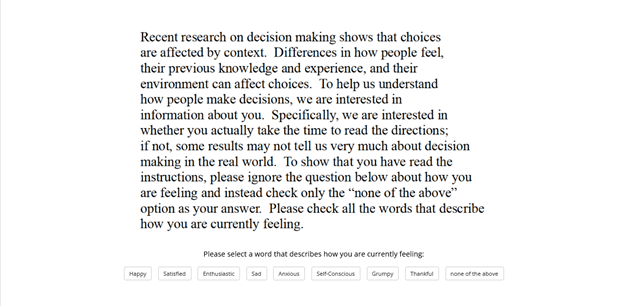
\includegraphics[width=6.25in,height=\textheight]{../resources/images/attention1a.png}
\caption{Screenshot of Attention Check}
\end{figure}

\begin{figure}
\centering
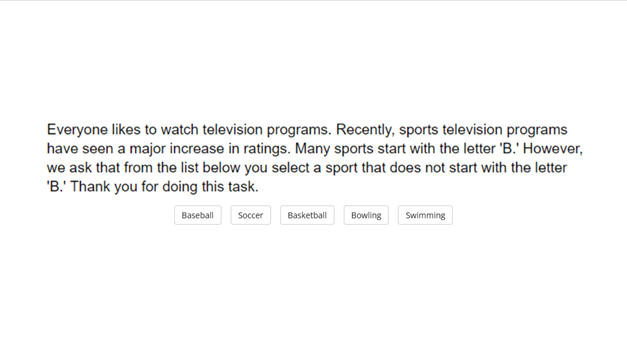
\includegraphics[width=5.20833in,height=\textheight]{../resources/images/attention2a.png}
\caption{Screenshot of Attention Check}
\end{figure}

~

\newpage

~

\newpage

\hypertarget{pilot-studies}{%
\section{Pilot Studies}\label{pilot-studies}}

Below we present a series of pilot studies (not pre-registered) in which we tested the feasibility of the paradigm using different cognitive load manipulations across different samples. In Studies S1 and S5 we used a sample of university students and a memory task involving an eight-digit number-letter string. In Studies S2 - S4 we used MTurk samples and a dot-pattern memory task.

The Studies below also provided a preliminary test of a secondary prediction of the dual-process explanation of moral dumbfounding. This second prediction is that responses in the dumbfounding paradigm will vary depending on individual differences. One individual difference variable linked to dual-process approaches to cognition, therefore may be related to susceptibility to dumbfounding is Need for Cognition (Cacioppo \& Petty, 1982; Forsterlee \& Ho, 1999; Petty, Cacioppo, \& Kao, 1984; Petty, Feinstein, Blair, \& Jarvis, 1996). The Need for Cognition Scale (NFC) is a measure of an individual's tendency ``to engage in and enjoy effortful analytic activity'' (Forsterlee \& Ho, 1999, p. 471; see also Cacioppo \& Petty, 1982), or a tendency to engage in deliberation (Evans \& Stanovich, 2013). We hypothesize that people who score high in NFC will be more likely to provide reasons for their judgment. Related to this, people who score low on the NFC are likely to fail to identify reasons for their judgment (or provide a dumbfounded response).

\newpage

\hypertarget{study-s1-number-letter-task-college-sample}{%
\section{Study S1: Number-Letter Task (College Sample)}\label{study-s1-number-letter-task-college-sample}}

The aim of Study S1 was to investigate if a cognitive load manipulation influenced participants' ability to justify their judgement. We also measured Need for Cognition (Cacioppo \& Petty, 1982; Petty et al., 1984) as a potential moderator variable.

\hypertarget{study-s1-method}{%
\subsection{Study S1: Method}\label{study-s1-method}}

\hypertarget{study-s1-participants-and-design}{%
\subsubsection{Study S1: Participants and design}\label{study-s1-participants-and-design}}

Study S1 was a between subjects design. The dependent variable was rates of providing reasons/dumbfounding (measured using to the critical slide with 3 response options: 1: providing reasons; 2: there is nothing wrong; 3: dumbfounded response - admission). The independent variable was cognitive load with two levels: present and absent. Cognitive load was manipulated by presenting participants with an eight digit number letter string to be memorized. Need for Cognition (Cacioppo \& Petty, 1982; Petty et al., 1984) was included as an additional potential predictor variable.

A total sample of 66 participants (55 female, 11 male; \emph{M}\textsubscript{age} = 22.42, min = 18, max = 57, \emph{SD} = 6.86) took part. Participants in this sample were undergraduate students, postgraduate students, and alumni from Mary Immaculate College (MIC), and University of Limerick (UL). Participation was voluntary and participants were not reimbursed for their participation.

\hypertarget{study-s1-procedure-and-materials}{%
\subsubsection{Study S1: Procedure and materials}\label{study-s1-procedure-and-materials}}

Data were collected using an online questionnaire. Data collection took place in a designated computer laboratory in MIC. The experimenter remained in the laboratory for the duration of the study. Participants were first presented with an information sheet and consent form. The main study proceeded when participants had signed the consent form.

Participants in the experimental condition were presented with an eight digit number/letter string and asked to memorise the sequence. After 30 seconds, the experiment progressed to the next slide. Participants had the option to click ``ok'' and progress to the next slide after 15 seconds.

Participants were then presented with the ``Julie and Mark'' (\emph{Incest}) vignette (Haidt, Björklund, \& Murphy, 2000). Participants rated on a 7-point Likert scale how right or wrong the behaviour of Julie and Mark was (where, 1 = \emph{Morally wrong}; 4 = \emph{neutral}; 7 = \emph{Morally right}), and were given an opportunity to provide reasons for their judgement. Following this, participants were presented with a series of counter-arguments, which refuted commonly used justifications for rating the behaviour as ``wrong''.

Dumbfounding was measured using the critical slide (McHugh et al., 2017). This contained a statement defending the behaviour and a question as to how the behaviour could be wrong (``Julie and Mark's behaviour did not harm anyone, how can there be anything wrong with what they did?''). There were three possible answer options: (a) ``There is nothing wrong''; (b) an admission of not having reasons (``It's wrong but I can't think of a reason''); and finally a judgement with accompanying justification (c) ``It's wrong and I can provide a valid reason''. The order of these response options was randomised. Participants who selected (c) were prompted to type a reason. The selecting of option (b), the admission of not having reasons, was taken to be a dumbfounded response. We note that this measure provides a conservative measure of dumbfounded responding (see McHugh et al., 2017 for discussion).

Following the critical slide, participants in the experimental condition were required to reproduce the eight digit number-letter string sequence presented previously. Following this a post-discussion questionnaire in which participants rated their response to the scenario across various dimensions (Haidt et al., 2000).

Need for Cognition was measured using the short form of the Need for Cognition scale (Cacioppo \& Petty, 1982; Petty et al., 1984). This is an 18 item scale containing questions relating to motivation to engage in thinking (e.g., ``I would prefer complex to simple problems''). Responses were recorded on a -4 to +4 Likert-type scale, where -4 = \emph{very strong disagreement} and +4 = \emph{very strong agreement}.

\hypertarget{study-s1-results}{%
\subsection{Study S1: Results}\label{study-s1-results}}

\begin{figure}[!h]
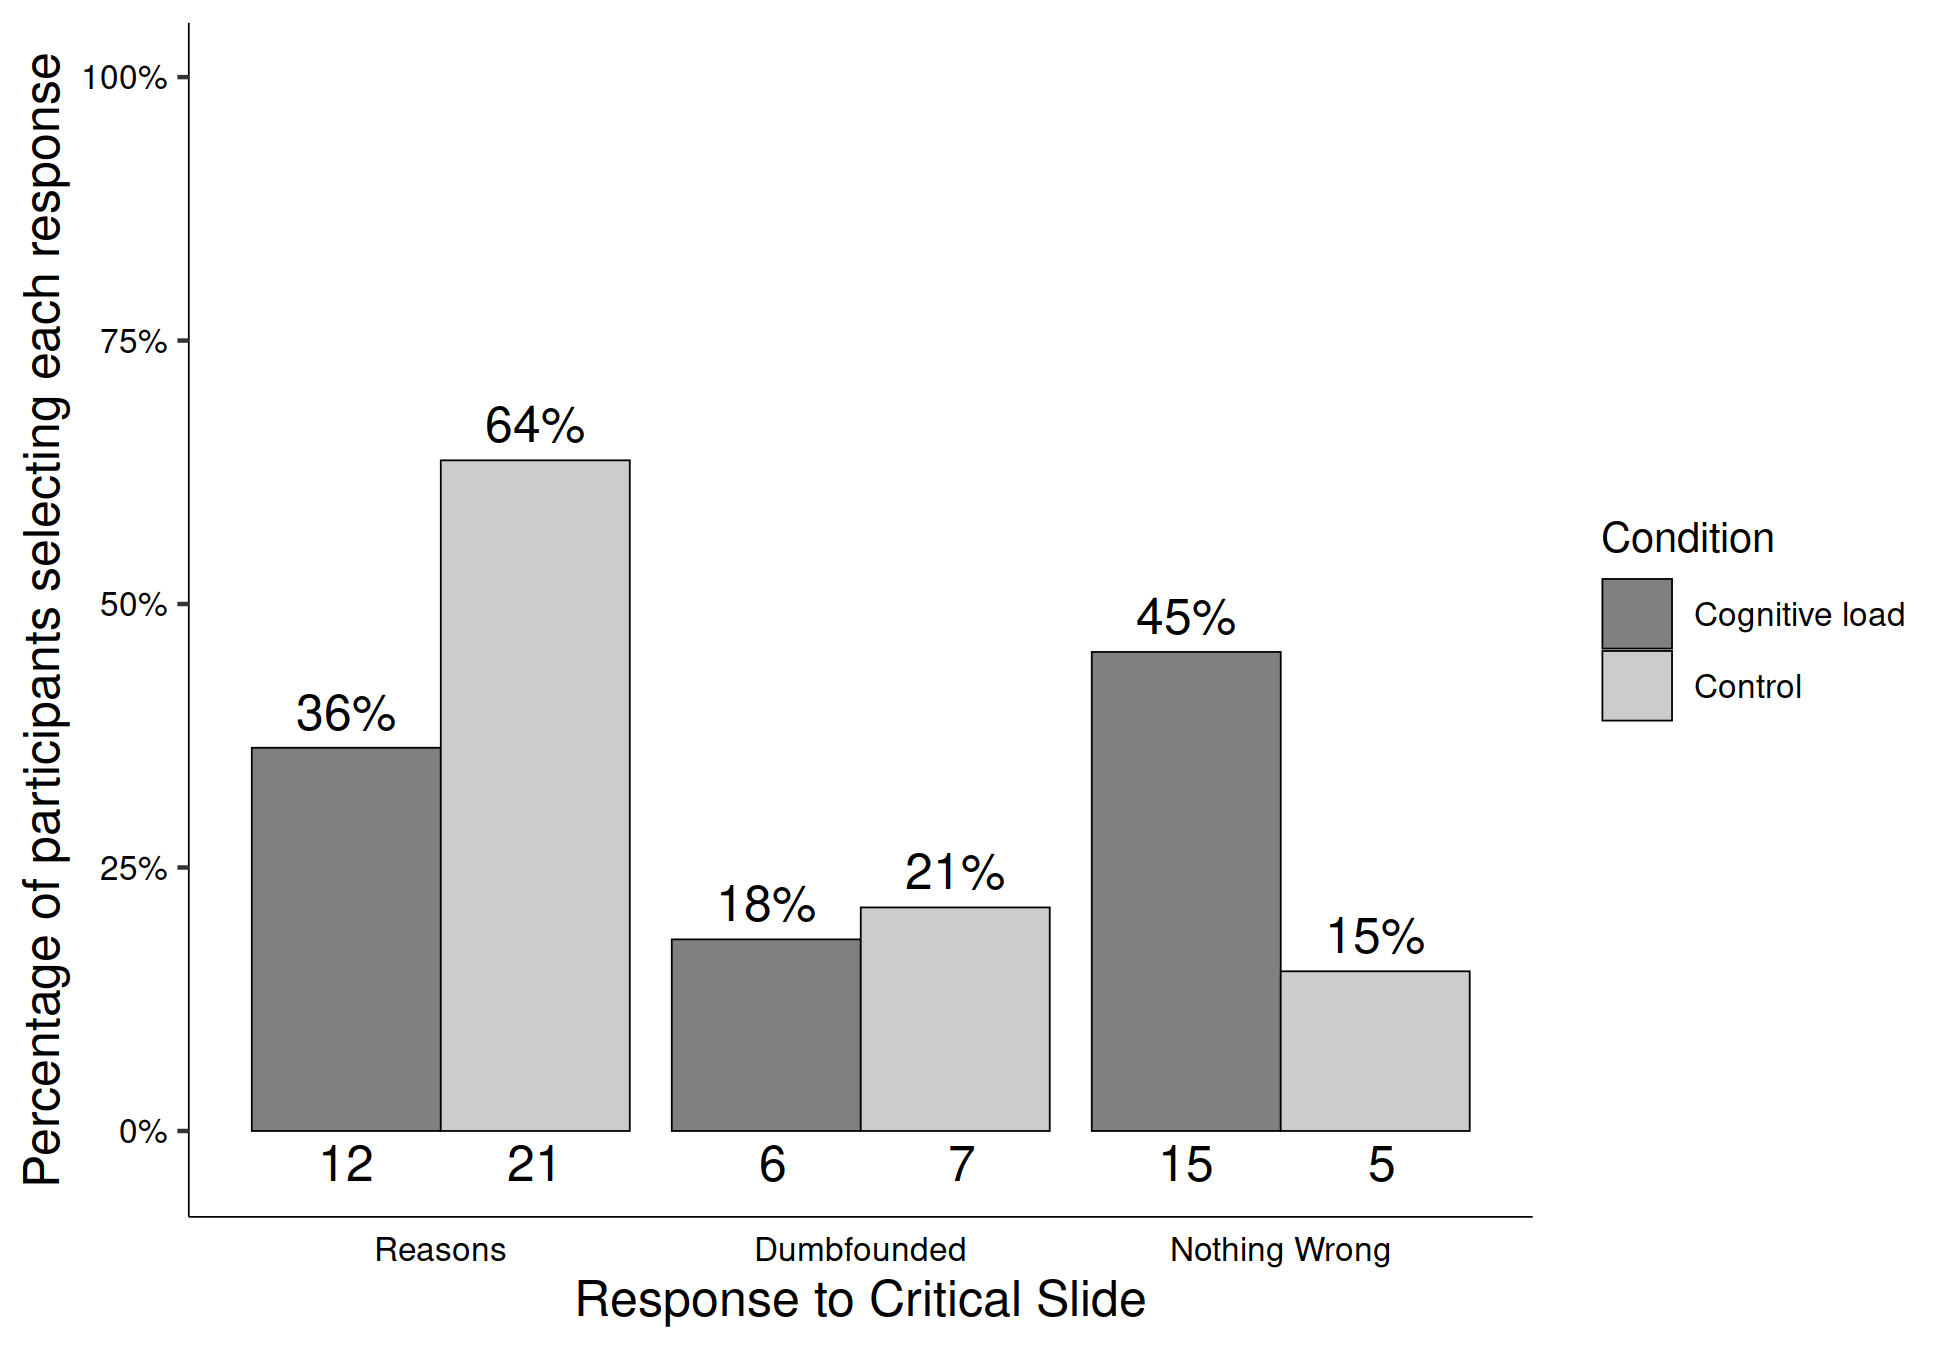
\includegraphics{Supplementary_files/figure-latex/S1S1fig2criticalcondition-1} \caption{Study S1: Responses to critical slide and for the experimental group (N = 33) and the control group (N = 33); (error bars represent standard error of the proportion)}\label{fig:S1S1fig2criticalcondition}
\end{figure}

\begin{figure}[!h]
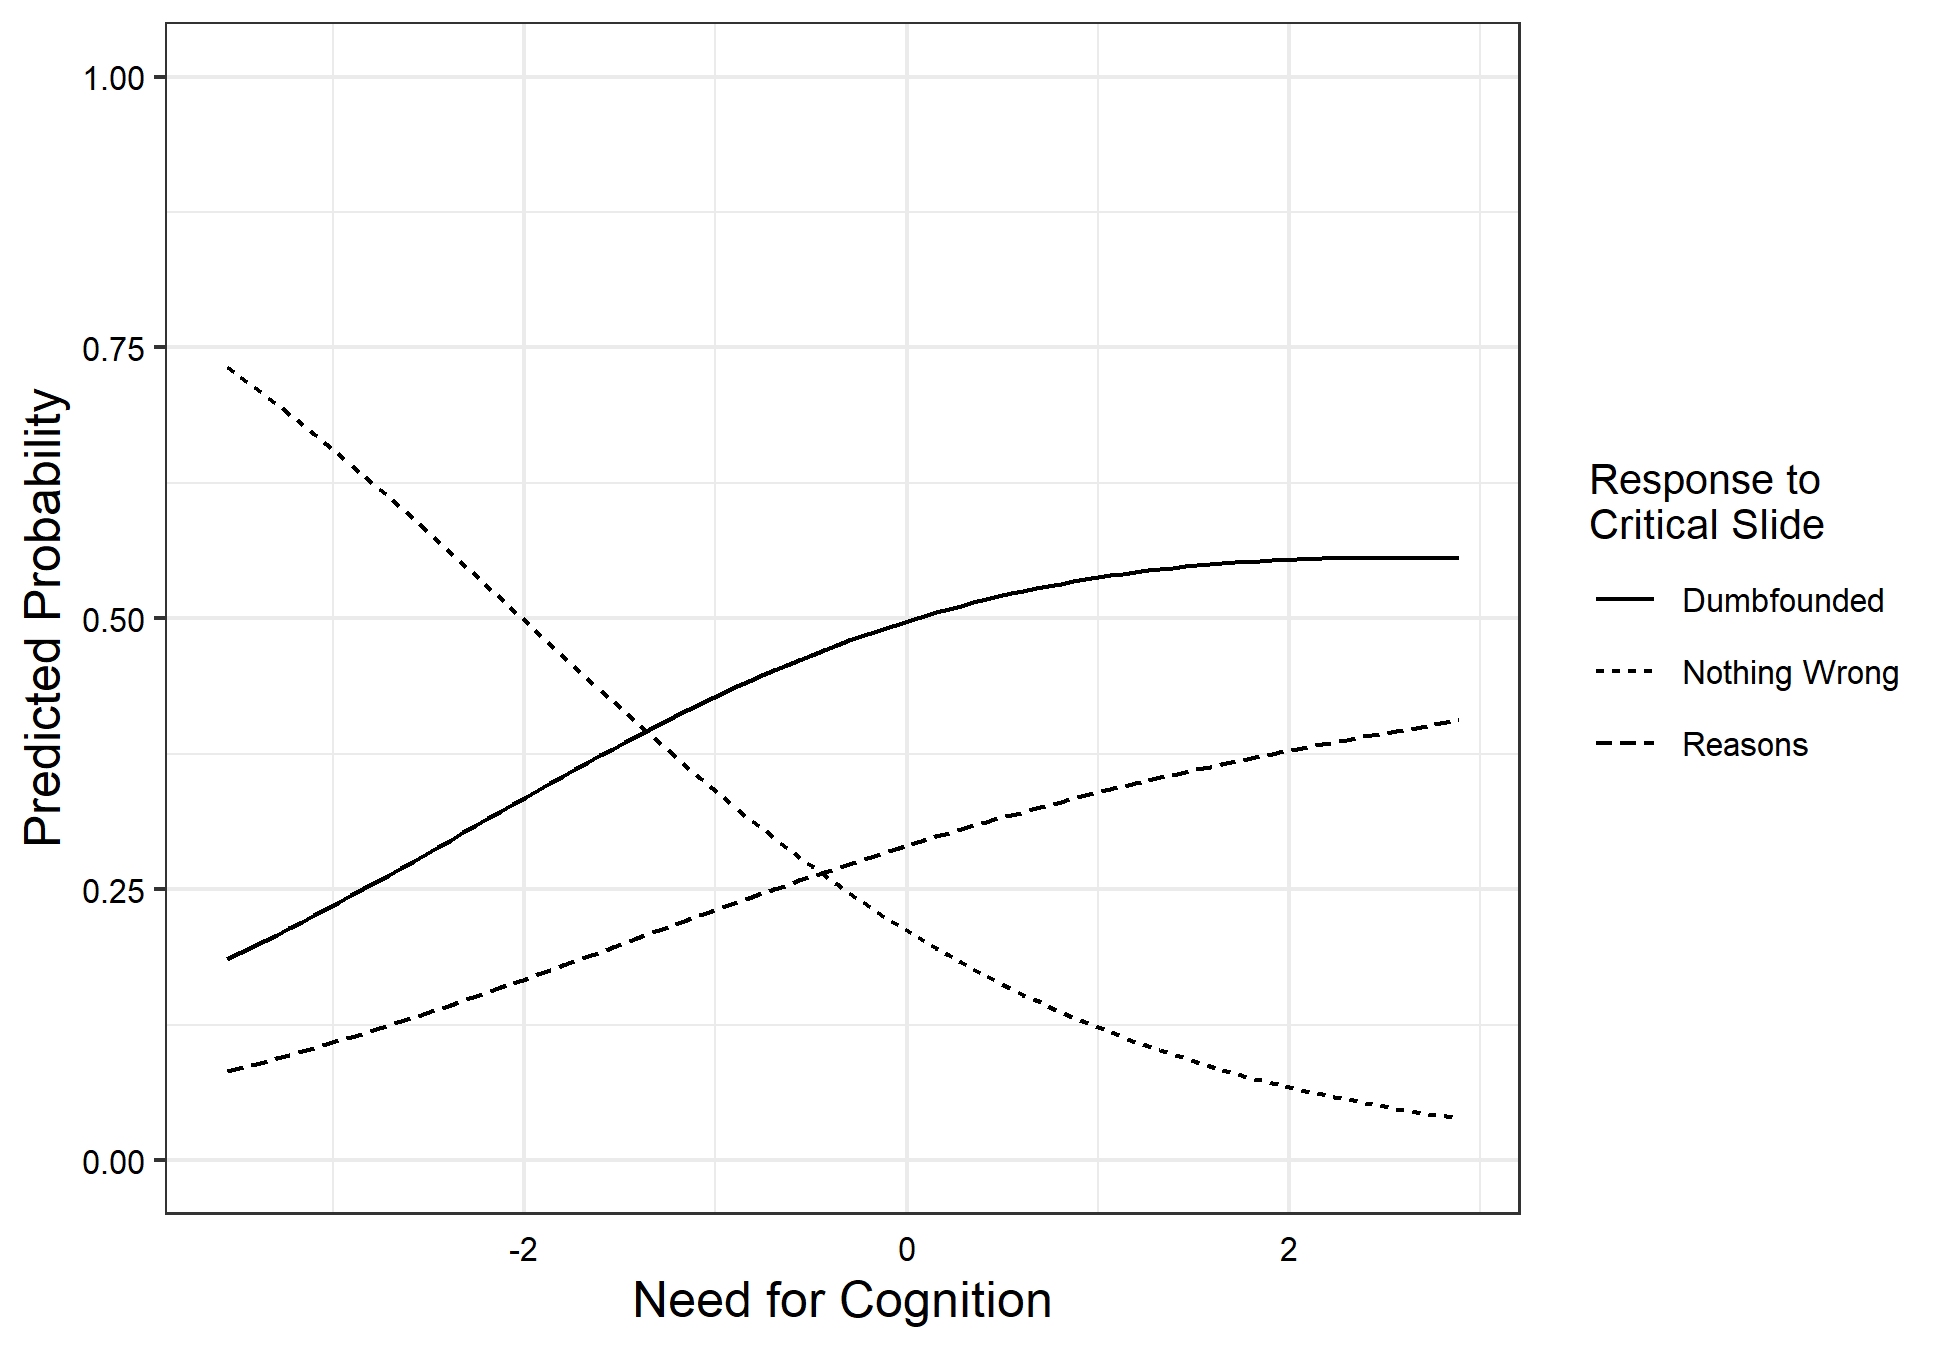
\includegraphics{Supplementary_files/figure-latex/S1ggplotlogit1-1} \caption{Study S1: Probability of selecting each response to the critical slide depending on Need for Cognition}\label{fig:S1ggplotlogit1}
\end{figure}

\newpage

\newpage

Forty six participants (69.70\%) rated the behavior of Julie and Mark as wrong initially, and forty one participants (62.12\%) rated the behavior as wrong at the end of the task. Initial ratings (\emph{M} = 2.38, \emph{SD} = 1.87) were significantly more severe than revised ratings (\emph{M} = 2.82, \emph{SD} = 1.91), \emph{t}(65) = -3.03, \emph{p} = .004; \emph{d} = 0.37. Inspection of the binned judgments revealed that twelve participants changed the valence of their judgments, and all but one of these involved included a ``neutral'' response for either the initial judgment or revised judgment Table~\ref{tab:tabS1change}.

\begin{table}[tbp]

\begin{center}
\begin{threeparttable}

\caption{\label{tab:tabS1change}Study S1 – Changes in Jugment}

\begin{tabular}{ccc}
\toprule
Initial Judgment & \multicolumn{1}{c}{Revised Judgment} & \multicolumn{1}{c}{Total Changed}\\
\midrule
neutral & right & 1\\
neutral & wrong & 3\\
wrong & neutral & 7\\
wrong & right & 1\\
\bottomrule
\end{tabular}

\end{threeparttable}
\end{center}

\end{table}

Participants who selected the admission of not having reasons on the critical slide were identified as dumbfounded. Thirteen participants (19.70\%) selected ``It's wrong but I can't think of a reason''. Thirty three participants (50\%) selected ``It's wrong and I can provide a valid reason''; and twenty participants (30.30\%) selected ``There is nothing wrong''.

\begin{table}[tbp]

\begin{center}
\begin{threeparttable}

\caption{\label{tab:tabS1tab1dumb1all}Study S1 – Response to the critical slide depending on cognitive load}

\begin{tabular}{lcccc}
\toprule
 & \multicolumn{2}{c}{Cognitive Load} & \multicolumn{2}{c}{Control} \\
\cmidrule(r){2-3} \cmidrule(r){4-5}
 & \multicolumn{1}{c}{N} & \multicolumn{1}{c}{\%} & \multicolumn{1}{c}{N} & \multicolumn{1}{c}{\%}\\
\midrule
It's wrong and I can provide a valid reason. & 12 & 36\% & 21 & 64\%\\
It's wrong but I can't think of a reason. & 6 & 18\% & 7 & 21\%\\
There is nothing wrong. & 15 & 45\% & 5 & 15\%\\
\bottomrule
\end{tabular}

\end{threeparttable}
\end{center}

\end{table}

Regarding the cognitive load manipulation, nine participants (27.27\%) successfully remembered the sequence of numbers and letters in full, and five participants (15.15\%) indicated they found the memory task easy. Of these, four participants both found the task easy and got the answer right. All participants correctly remembered at least two digits, indicating at least some level of engagement with the cognitive load manipulation. There were no differences in initial judgement, \emph{t}(63.90) = 1.26, \emph{p} = .214; \emph{d} = 0.31, or revised judgment, \emph{t}(63.99) = 1.16, \emph{p} = .250; \emph{d} = 0.29, depending on cognitive load.

To test our main hypotheses we conducted a chi-squared test for independence which revealed a significant association between experimental condition and response to the critical slide, \(\chi\)\textsuperscript{2}(2, \emph{N} = 66) = 7.53, \emph{p} = .023, \emph{V} = 0.34, the observed power was 0.69. Under cognitive load fewer participants (12; 36.36\%) provided reasons than in the control condition (21; 63.64\%). Similarly, under cognitive load more participants (15; 45.45\%) selected ``There is nothing wrong'' than in the control group (5; 15.15\%). The responses to the critical slide for the experimental group (\emph{N} = 33) and the control group (\emph{N} = 33) are displayed in Figure~\ref{fig:S1S1fig2criticalcondition} and Table~\ref{tab:tabS1tab1dumb1all}. The observed counts, expected counts and standardised residuals are displayed in Table~\ref{tab:S1tab1dumb}.

\begin{table}[tbp]

\begin{center}
\begin{threeparttable}

\caption{\label{tab:S1tab1dumb}Study S1 – Observed counts, expected counts, and standardised residuals for each response to the critical slide depending on cognitive load}

\begin{tabular}{llcc}
\toprule
 & \multicolumn{1}{c}{} & \multicolumn{1}{c}{Cognitive Load} & \multicolumn{1}{c}{Control}\\
\midrule
Observed count & Reasons & 12 & 21\\
 & Dumbfounded & 6 & 7\\
 & Nothing Wrong & 15 & 5\\
Expected count & Reasons & 16.5 & 16.5\\
 & Dumbfounded & 6.5 & 6.5\\
 & Nothing Wrong & 10 & 10\\
Standardised residuals & Reasons & -2.22* & 2.22*\\
 & Dumbfounded & -0.31 & 0.31\\
 & Nothing Wrong & 2.68* & -2.68*\\
\bottomrule
\addlinespace
\end{tabular}

\begin{tablenotes}[para]
\normalsize{\textit{Note.} * = sig. at \emph{p} < .05; ** = sig. at \emph{p} < .001}
\end{tablenotes}

\end{threeparttable}
\end{center}

\end{table}

A multinomial logistic regression revealed no significant association between Need for Cognition and response to the critical slide, \(\chi\)\textsuperscript{2}(2, \emph{N} = 66) = 4.86, \emph{p} = .088, the observed power was 0.49.

\newpage

\newpage

\hypertarget{study-s2-dot-pattern-task-online-sample}{%
\section{Study S2: Dot-Pattern Task (Online Sample)}\label{study-s2-dot-pattern-task-online-sample}}

Study S1 demonstrated interesting variability in responses to the critical slide depending on cognitive load. The aim of Study S2 was to assess the replicability of the results of Study S1, using an online sample. In Study S1, the experimenter was in the room with the participants. This made it more difficult for participants to cheat on the memory task. This is not possible with an online sample. An alternative cognitive load manipulation was taken from De Neys and Schaeken (De Neys \& Schaeken, 2007), whereby a dot pattern is briefly presented to participants, and participants are required to reproduce the dot pattern at a later stage.

\hypertarget{study-s2-method}{%
\subsection{Study S2: Method}\label{study-s2-method}}

\hypertarget{study-s2-participants-and-design}{%
\subsubsection{Study S2: Participants and design}\label{study-s2-participants-and-design}}

Study S2 was a between subjects design. The dependent variable was response to the critical slide. The independent variable was cognitive load with two levels: high and low. Need for Cognition (Cacioppo \& Petty, 1982; Petty et al., 1984) was included as a potential correlate and moderator variable.

A total sample of 100 participants (56 female, 44 male; \emph{M}\textsubscript{age} = 38.38, min = 19, max = 72, \emph{SD} = 12.41) took part. Participants in this sample were recruited using Amazon's MTurk (Amazon Web Services Inc., 2016). Participants were paid \$0.50 for their participation. Participants were recruited from English speaking countries or from countries where residents generally have a high level of English (e.g., The Netherlands, Denmark, Sweden).

\hypertarget{study-s2-procedure-and-materials}{%
\subsubsection{Study S2: Procedure and materials}\label{study-s2-procedure-and-materials}}

Data were collected using an online questionnaire. Materials were largely the same as in Study S1, with a change to the cognitive load manipulation. Cognitive load was manipulated using a dot-pattern memory task (De Neys \& Schaeken, 2007).

Participants were presented with a 3 x 3 grid containing a dot pattern. This image disappeared after one second. Participants then answered a question relating to the moral judgement task. Following this, participants were asked to reproduce the dot-pattern. All participants took part in the memory task, and cognitive load was manipulated by varying the complexity of the patterns presented (De Neys \& Schaeken, 2007). The control group were presented with simple patterns, containing three dots in a line, while the experimental group were presented with more complex dot patterns containing 4 dots, see Figure~\ref{fig:S2dotpattern}.

\begin{figure}[!h]
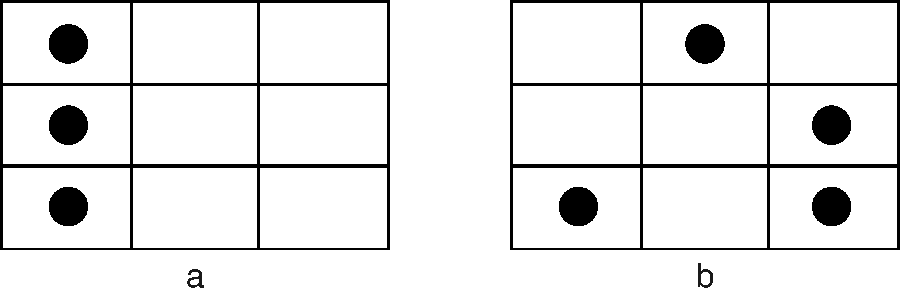
\includegraphics{Supplementary_files/figure-latex/S2dotpattern-1} \caption{Sample dot patterns - more simple for the control group (a) and higher complexity for the experimental condition (b)}\label{fig:S2dotpattern}
\end{figure}

Study S2 proceeded in much the same way as Study S1. There were four target questions during which participants were engaged in the memory task. A different pattern was presented before each of the following: the initial judgement, the initial opportunity to provide reasons, the critical slide, and the revised judgement. After each of these questions participants were required to reproduce the pattern. As in Study S1, dumbfounding was measured using the critical slide.

\hypertarget{study-s2-results}{%
\subsection{Study S2: Results}\label{study-s2-results}}

Seventy seven participants (77\%) rated the behavior of Julie and Mark as wrong initially, and seventy participants (70\%) rated the behavior as wrong at the end of the task. Initial ratings (\emph{M} = 2.13, \emph{SD} = 1.54) were significantly more severe than revised ratings (\emph{M} = 2.35, \emph{SD} = 1.65), \emph{t}(99) = -2.85, \emph{p} = .005; \emph{d} = 0.28. Inspection of the binned judgments revealed that ten participants changed the valence of their judgments, and all but one of these involved one judgment that was neutral (see Table~\ref{tab:tabS2change}).

\begin{table}[tbp]

\begin{center}
\begin{threeparttable}

\caption{\label{tab:tabS2change}Study S2 – Changes in Jugment}

\begin{tabular}{ccc}
\toprule
Initial Judgment & \multicolumn{1}{c}{Revised Judgment} & \multicolumn{1}{c}{Total Changed}\\
\midrule
neutral & right & 2\\
right & neutral & 1\\
wrong & neutral & 6\\
wrong & right & 1\\
\bottomrule
\end{tabular}

\end{threeparttable}
\end{center}

\end{table}

Participants who selected the admission of not having reasons on the critical slide were identified as dumbfounded. Twenty six participants (26\%) selected ``It's wrong but I can't think of a reason''. Fifty participants (50\%) selected ``It's wrong and I can provide a valid reason''; and twenty four participants (24\%) selected ``There is nothing wrong''.

A chi-squared test for independence revealed no association between experimental condition and response to the critical slide, \(\chi\)\textsuperscript{2}(6, \emph{N} = 100) = 1.36, \emph{p} = .968, \emph{V} = 0.09, the observed power was 0.11. The responses to the critical slide for the experimental group (\emph{N} = 51) and the control group (\emph{N} = 49) are displayed in Figure~\ref{fig:S2figboth} and Table~\ref{tab:tabS2tab1dumb1all}.

\begin{table}[tbp]

\begin{center}
\begin{threeparttable}

\caption{\label{tab:tabS2tab1dumb1all}Study S2 – Response to the critical slide depending on cognitive load/engagement}

\begin{tabular}{llcccc}
\toprule
 &  & \multicolumn{2}{c}{Cognitive Load} & \multicolumn{2}{c}{Control} \\
\cmidrule(r){3-4} \cmidrule(r){5-6}
Measure & \multicolumn{1}{c}{Response} & \multicolumn{1}{c}{N} & \multicolumn{1}{c}{\%} & \multicolumn{1}{c}{N} & \multicolumn{1}{c}{\%}\\
\midrule
Manipulation Only & Reasons & 25 & 49\% & 25 & 51\%\\
 & Dumbfounded & 15 & 29\% & 11 & 22\%\\
 & Nothing Wrong & 11 & 22\% & 13 & 27\%\\
Engagement & Reasons & 23 & 41\% & 27 & 61\%\\
 & Dumbfounded & 20 & 36\% & 6 & 14\%\\
 & Nothing Wrong & 13 & 23\% & 11 & 25\%\\
\bottomrule
\end{tabular}

\end{threeparttable}
\end{center}

\end{table}

\begin{figure}[!h]
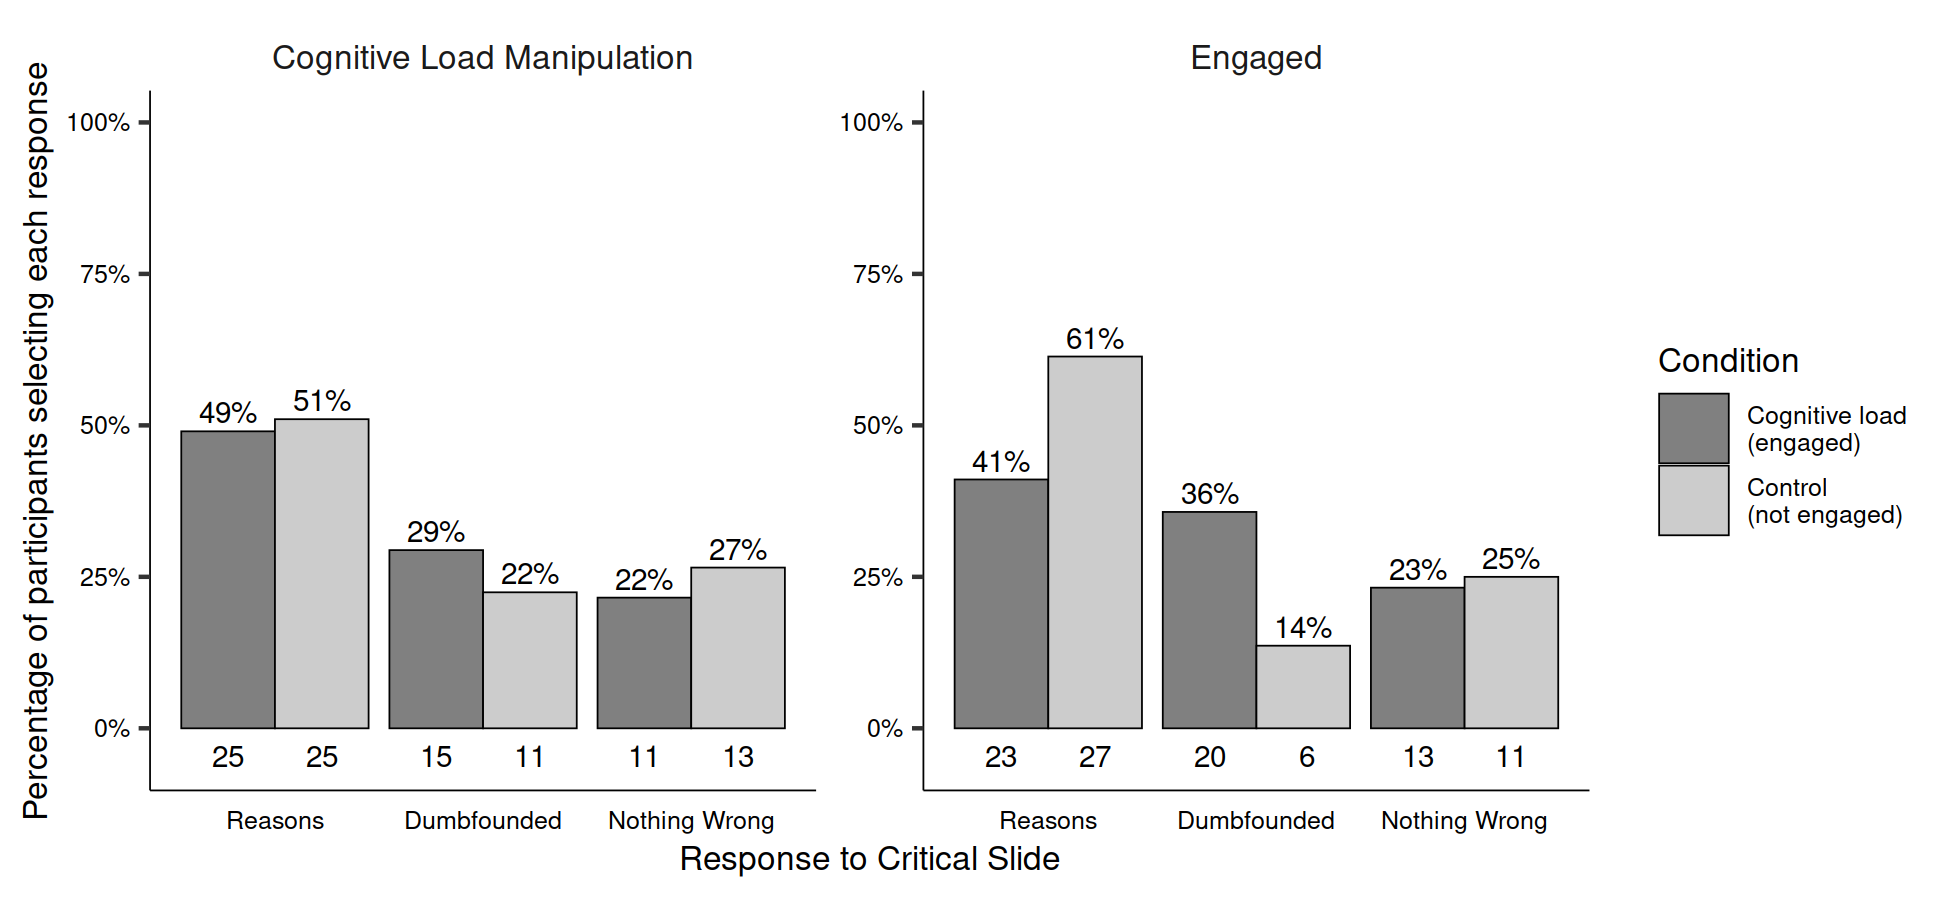
\includegraphics{Supplementary_files/figure-latex/S2figboth-1} \caption{Study S2: Responses to critical slide for (left) the experimental group (N = 51) vs the control group (N = 49); and (right) depending on engagement (N = 56) or non-engagement (N = 44) with the memory task (error bars represent standard error of the proportion)}\label{fig:S2figboth}
\end{figure}

\begin{figure}[!h]
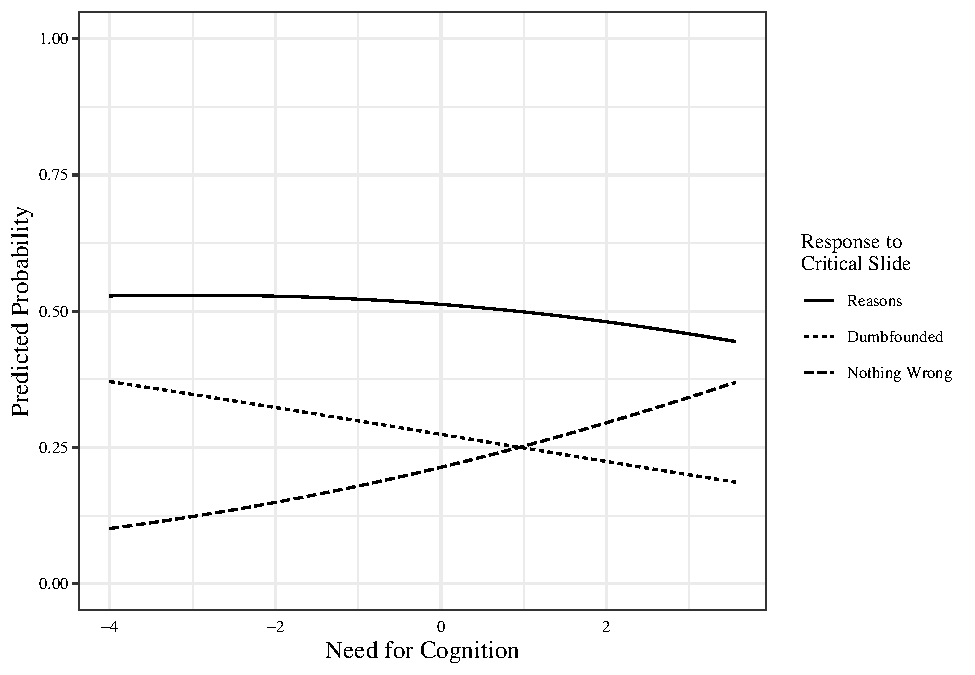
\includegraphics{Supplementary_files/figure-latex/S2ggplotlogit2-1} \caption{Study S2: Probability of selecting each response to the critical slide depending on Need for Cognition}\label{fig:S2ggplotlogit2}
\end{figure}

It is possible that the difference in results observed between Study S1 and Study S2 is due to the alternative manipulation of cognitive load employed. In Study S1, the control group did not engage in any task, however, adopting De Neys and Shaeken's procedure (2007), participants in the control group of Study S2 engaged in a memory task. It is possible that simply engaging in a memory task led to differences in responses, and that level of difficulty (the manipulation that was employed) was irrelevant. Indeed, the responding to the critical slide in the control group in Study S2 is more similar to the responding in the experimental group in 1 than to the control group in Study S1. Furthermore, rates of successful reproduction of the dot patterns in Study S2 were much lower than reported by De Neys and Shaeken (2007). It is likely that engagement with the memory task in Study S2 was not comparable to that observed by De Neys and Shaeken (2007), and this impacted the results. We propose that not engaging appropriately with the memory task undermines its efficacy as a cognitive load manipulation, and hypothesized that the effect of the cognitive load manipulation is related to the degree to which people engage with the manipulation.

\begin{table}[tbp]

\begin{center}
\begin{threeparttable}

\caption{\label{tab:S2S2tab1dumb}Study S2 – Observed counts, expected counts, and standardised residuals for each response to the critical slide depending on cognitive load}

\begin{tabular}{llcc}
\toprule
 & \multicolumn{1}{c}{} & \multicolumn{1}{c}{Engaged} & \multicolumn{1}{c}{Not Engaged}\\
\midrule
Observed count & Reasons & 23 & 27\\
 & Dumbfounded & 20 & 6\\
 & Nothing Wrong & 13 & 11\\
Expected count & Reasons & 28 & 22\\
 & Dumbfounded & 14.56 & 11.44\\
 & Nothing Wrong & 13.44 & 10.56\\
Standardised residuals & Reasons & -2.01* & 2.01*\\
 & Dumbfounded & 2.5* & -2.5*\\
 & Nothing Wrong & -0.21 & 0.21\\
\bottomrule
\addlinespace
\end{tabular}

\begin{tablenotes}[para]
\normalsize{\textit{Note.} * = sig. at \emph{p} < .05; ** = sig. at \emph{p} < .001}
\end{tablenotes}

\end{threeparttable}
\end{center}

\end{table}

To test this claim we developed a measure of engagement with the memory task. The memory task involved correctly placing dots in a 3 x 3 grid. For the scoring of this task, each of the nine places in the grid could be marked/not marked correctly or incorrectly, making 9 the total possible number of correct responses. If a person misplaced one dot in the pattern this would count for 2 incorrect places in the grid: the mark in the incorrect place, and the absence of a mark in the place it should have been. A participant who received a score of 7, could reasonably be taken to have engaged with the task, and simply made a slip. As such, this was taken as the cut-off point for identifying engagement. This resulted in 56 participants being identified as engaging with the memory task, and 44 being identified as not engaging with the task.

Using this engagement threshold, we tested if responses to the critical were associated with engagement with the memory task. A chi-squared test for independence revealed an association between engagement in the memory task and response to the critical slide, \(\chi\)\textsuperscript{2}(2, \emph{N} = 100) = 6.68, \emph{p} = .035, \emph{V} = 0.26, the observed power was 0.11. The responses to the critical slide for the experimental group (\emph{N} = 51) and the control group (\emph{N} = 49) are displayed in Figure~\ref{fig:S2figboth}. The observed counts, expected counts and standardized residuals are displayed in Table~\ref{tab:S2S2tab1dumb}.

A multinomial logistic regression revealed no significant association between Need for Cognition and response to the critical slide, \(\chi\)\textsuperscript{2}(2, \emph{N} = 100) = 2.19, \emph{p} = .334, the observed power was 0.24 (see Figure~\ref{fig:S2ggplotlogit2} for relative probabilities of selecting each response depending on Need for Cognition).

\newpage

\hypertarget{study-s3-dot-pattern---controlling-for-engagement-online-sample}{%
\section{Study S3: Dot-Pattern - Controlling for Engagement (Online Sample)}\label{study-s3-dot-pattern---controlling-for-engagement-online-sample}}

In Study S2 the role of engagement with the memory task emerged as an important moderator of the effectiveness of the cognitive load manipulation. Study S3 was conducted in order to test if cognitive load affects participants' ability to identify reasons for their judgement, when accounting for engagement with the memory task. We therefore only included participants in our analysis who engaged with the memory task while completing the critical slide (evidenced by a score of 7 or higher). As above, our hypothesis is that participants engaging in this memory task will be less likely to provide reasons than participants in the control group.

\hypertarget{study-s3-methods}{%
\subsection{Study S3: Methods}\label{study-s3-methods}}

\hypertarget{study-s3-participants-and-design}{%
\subsubsection{Study S3: Participants and Design}\label{study-s3-participants-and-design}}

Study S3 was a between subjects design. The dependent variable was response to the critical slide. The independent variable was cognitive load with two levels: present and absent. Need for Cognition (Cacioppo \& Petty, 1982; Petty et al., 1984) was included as a potential correlate and moderator variable.

Following the elimination of 34 participants who scored less than 7 on the memory task we were left with a final sample of 129 participants (74 female, 55 male; \emph{M}\textsubscript{age} = 40.26, min = 20, max = 72, \emph{SD} = 13.04). Participants in this sample were recruited through MTurk (under the same conditions as Study S2).

\hypertarget{study-s3-procedure-and-materials}{%
\subsubsection{Study S3: Procedure and Materials}\label{study-s3-procedure-and-materials}}

Study S3 was the same as Study S2 with two changes. The control group did not take part in a memory task, and to avoid task fatigue, in the dot patterns presented to the experimental group, the dot patterns presented alternated between the easy 3-dot patterns and the complex 4-dot patterns.

A score of 7 or higher on the memory task that accompanied the critical slide was selected as the measure of engagement with the memory task. Only participants who engaged with the task were eligible for analysis. Other than the two changes described above, Study S3 was the same as Study S2.

\hypertarget{study-s3-results}{%
\subsection{Study S3: Results}\label{study-s3-results}}

\begin{figure}[!h]
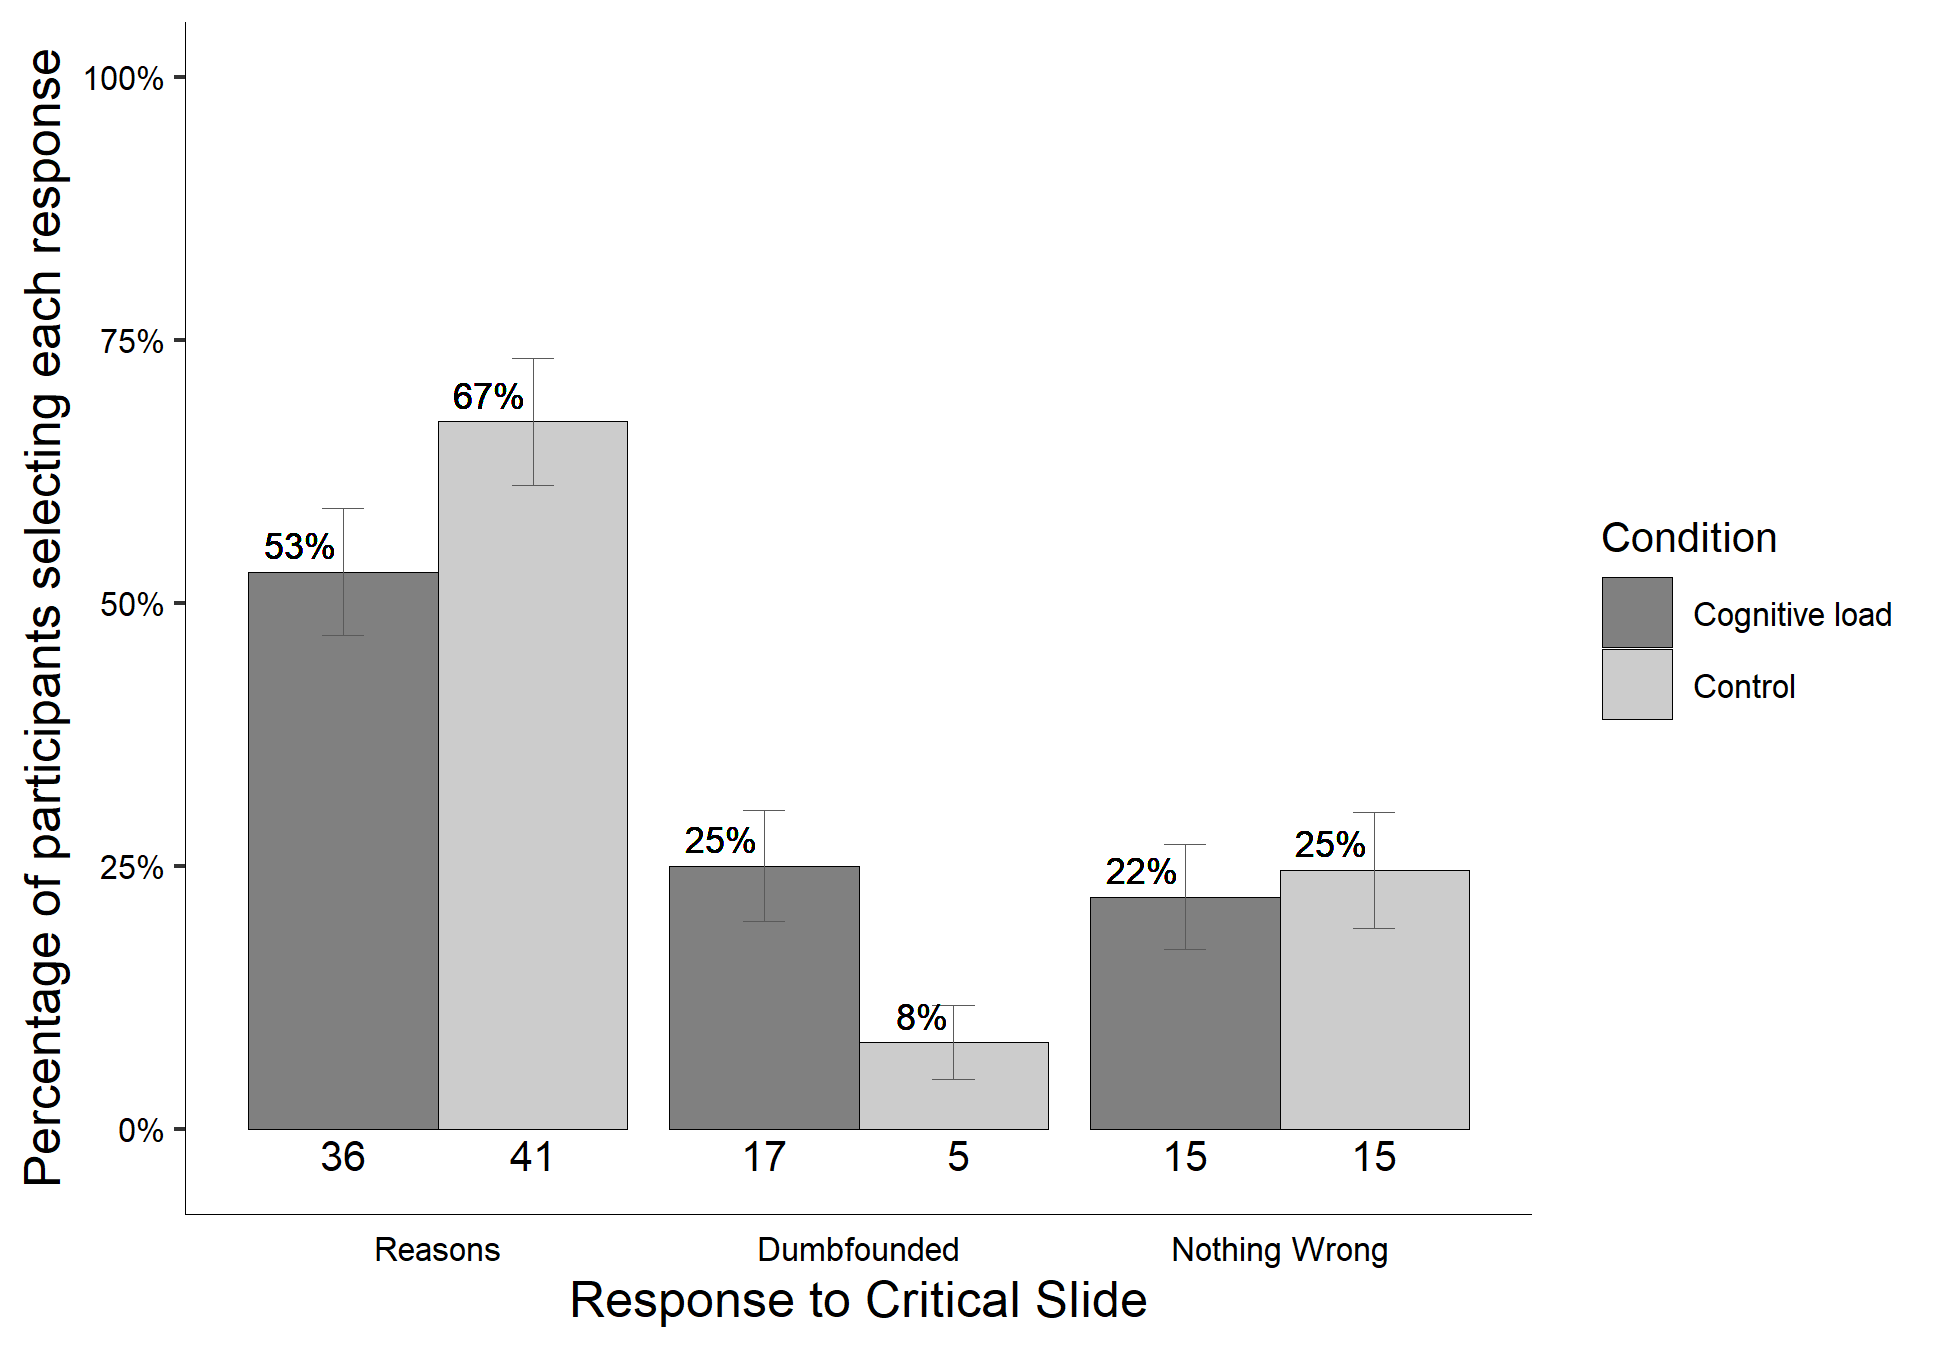
\includegraphics{Supplementary_files/figure-latex/S3ch5S3fig2criticalcondition-1} \caption{Study S3: Responses to critical slide for the cognitive load group (N = 68) and the control group (N = 61); (error bars represent standard error of the proportion)}\label{fig:S3ch5S3fig2criticalcondition}
\end{figure}

\begin{figure}[!h]
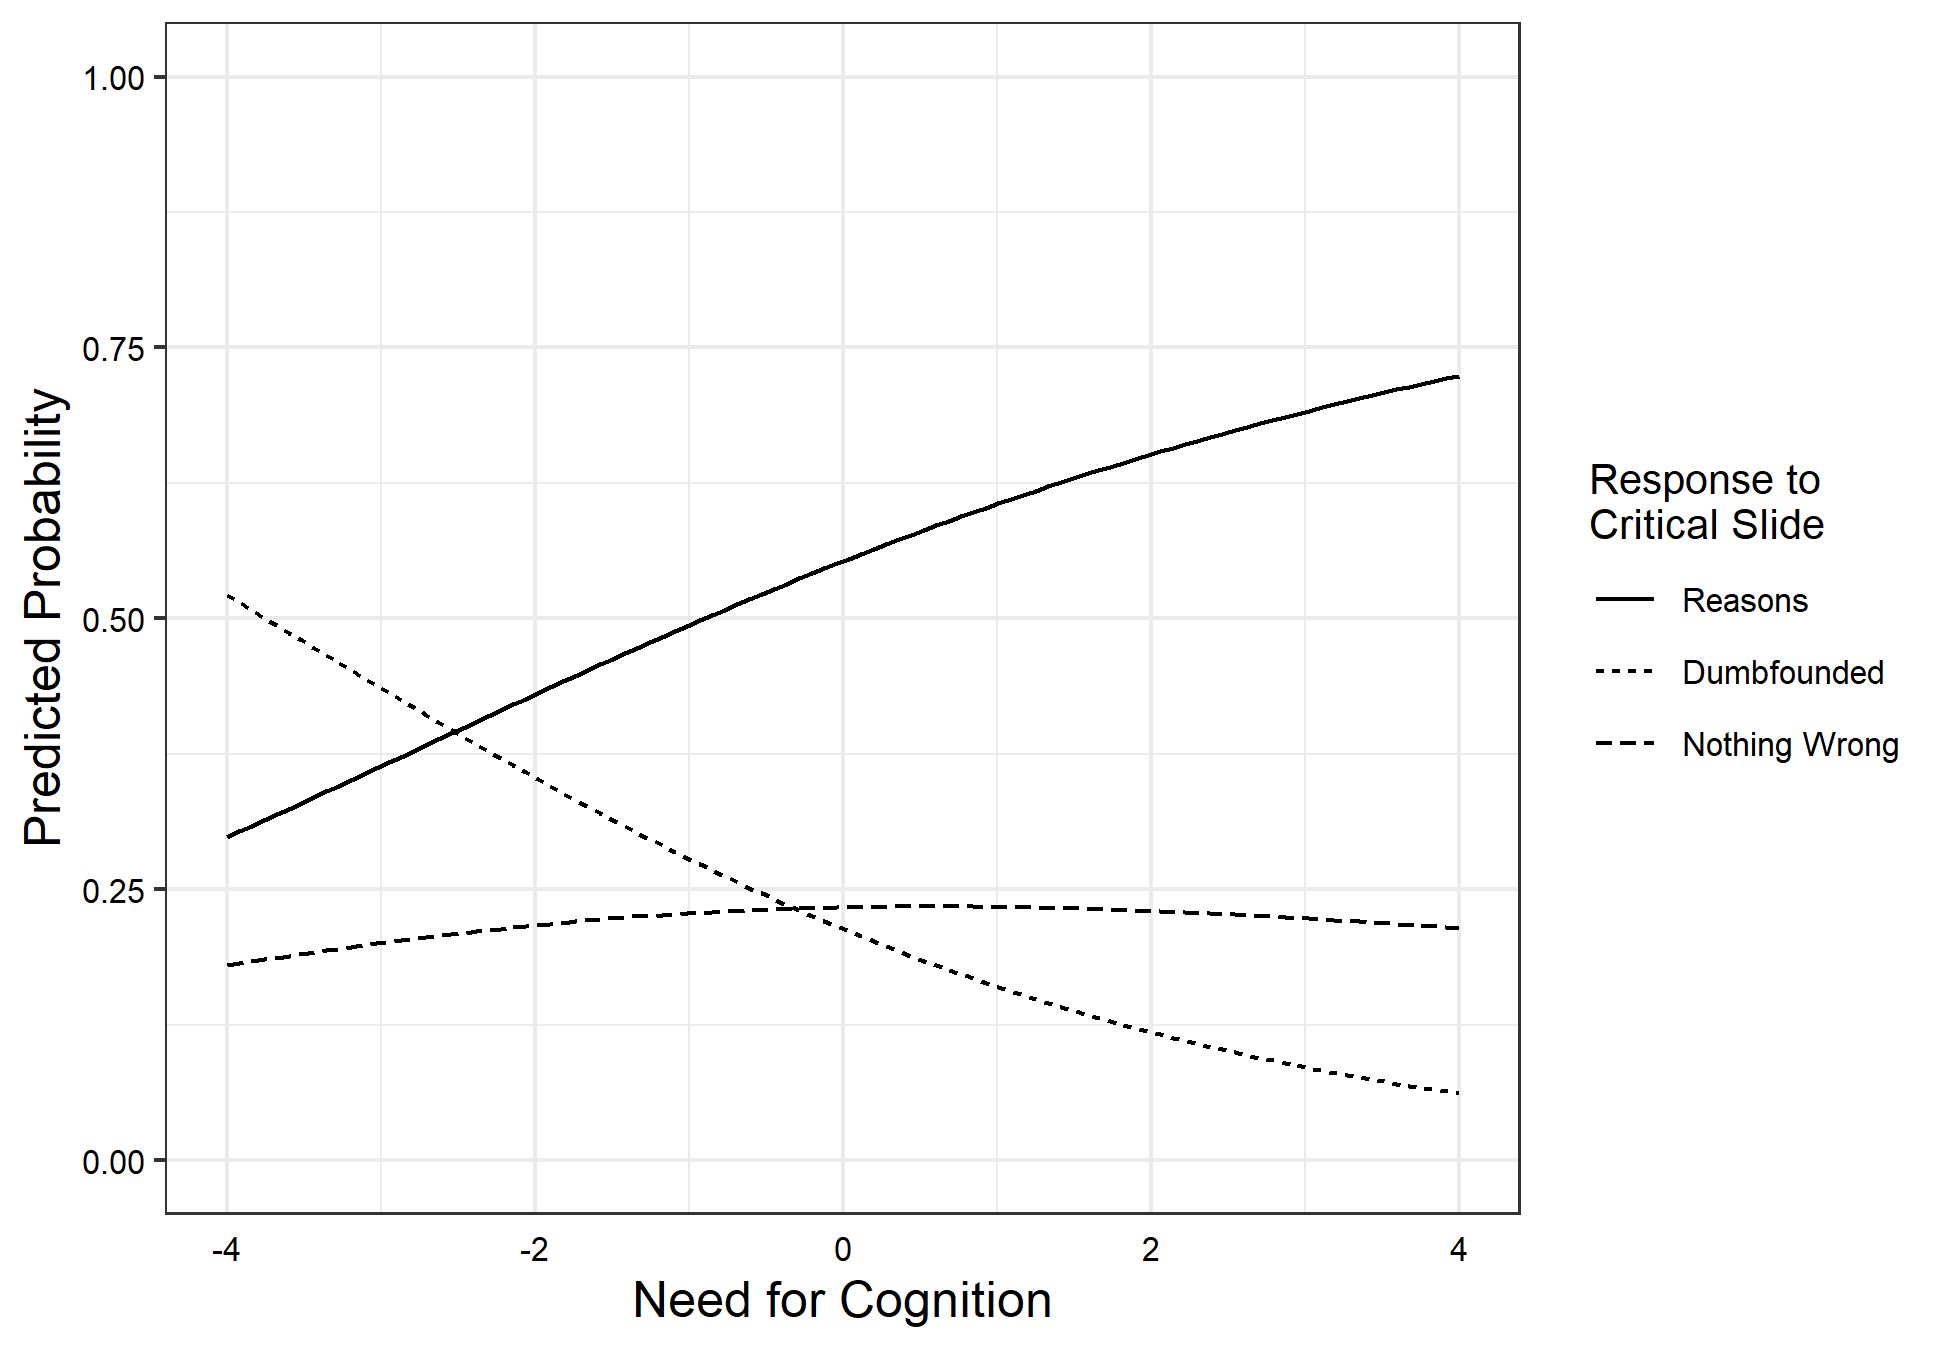
\includegraphics{Supplementary_files/figure-latex/S3ggplotlogit3-1} \caption{Study S3: Probability of selecting each response to the critical slide depending on Need for Cognition}\label{fig:S3ggplotlogit3}
\end{figure}

Ninety four participants (74.02\%) rated the behavior of Julie and Mark as wrong initially, and ninety three participants (73.23\%) rated the behavior as wrong at the end of the task. Initial ratings (\emph{M} = 2.26, \emph{SD} = 1.76) were significantly more severe than revised ratings (\emph{M} = 2.34, \emph{SD} = 1.75), \emph{t}(126) = -1.15, \emph{p} = .253; \emph{d} = 0.10. Inspection of the binned judgments revealed that thirteen participants changed the valence of their judgments, and all but three of these involved one judgment that was neutral (see Table~\ref{tab:tabS3change}).

\begin{table}[tbp]

\begin{center}
\begin{threeparttable}

\caption{\label{tab:tabS3change}Study S3 – Changes in Jugment}

\begin{tabular}{ccc}
\toprule
Initial Judgment & \multicolumn{1}{c}{Revised Judgment} & \multicolumn{1}{c}{Total Changed}\\
\midrule
neutral & right & 2\\
neutral & wrong & 2\\
right & neutral & 4\\
right & wrong & 1\\
wrong & neutral & 2\\
wrong & right & 2\\
\bottomrule
\end{tabular}

\end{threeparttable}
\end{center}

\end{table}

Turning to responses to the critical slide, twenty two participants (17.32\%) selected ``It's wrong but I can't think of a reason''. Seventy six participants (59.84\%) selected ``It's wrong and I can provide a valid reason''; and twenty nine participants (22.83\%) selected ``There is nothing wrong''.

\begin{table}[tbp]

\begin{center}
\begin{threeparttable}

\caption{\label{tab:tabS3tab1dumb1all}Study S3 – Response to the critical slide depending on cognitive load/engagement}

\begin{tabular}{llccc}
\toprule
 & \multicolumn{2}{c}{Cognitive Load} & \multicolumn{2}{c}{Control} \\
\cmidrule(r){2-3} \cmidrule(r){4-5}
 & \multicolumn{1}{c}{N} & \multicolumn{1}{c}{\%} & \multicolumn{1}{c}{N} & \multicolumn{1}{c}{\%}\\
\midrule
It's wrong and I can provide a valid reason. & 36 & 54\% & 40 & 67\%\\
It's wrong but I can't think of a reason. & 17 & 25\% & 5 & 8\%\\
There is nothing wrong. & 14 & 21\% & 15 & 25\%\\
\bottomrule
\end{tabular}

\end{threeparttable}
\end{center}

\end{table}

\newpage

\begin{table}[tbp]

\begin{center}
\begin{threeparttable}

\caption{\label{tab:S3S3tab1dumb}Study S3 – Observed counts, expected counts, and standardised residuals for each response to the critical slide depending on cognitive load}

\begin{tabular}{llcc}
\toprule
 & \multicolumn{1}{c}{} & \multicolumn{1}{c}{Cognitive Load} & \multicolumn{1}{c}{Control}\\
\midrule
Observed count & Reasons & 36 & 40\\
 & Dumbfounded & 17 & 5\\
 & Nothing Wrong & 14 & 15\\
Expected count & Reasons & 40.09 & 35.91\\
 & Dumbfounded & 11.61 & 10.39\\
 & Nothing Wrong & 15.3 & 13.7\\
Standardised residuals & Reasons & -1.48 & 1.48\\
 & Dumbfounded & 2.53* & -2.53*\\
 & Nothing Wrong & -0.55 & 0.55\\
\bottomrule
\addlinespace
\end{tabular}

\begin{tablenotes}[para]
\normalsize{\textit{Note.} * = sig. at \emph{p} < .05; ** = sig. at \emph{p} < .001}
\end{tablenotes}

\end{threeparttable}
\end{center}

\end{table}

A chi-squared test for independence revealed a significant association between experimental condition and response to the critical slide, \(\chi\)\textsuperscript{2}(2, \emph{N} = 127) = 6.42, \emph{p} = .040, \emph{V} = 0.22, the observed power was 0.62. The responses to the critical slide for the experimental group (\emph{N} = 67) and the control group (\emph{N} = 60) are displayed in Figure~\ref{fig:S3ch5S3fig2criticalcondition} Table~\ref{tab:tabS3tab1dumb1all}. The observed counts, expected counts and standardised residuals are displayed in Table~\ref{tab:S3S3tab1dumb}.

\newpage

A multinomial logistic regression revealed a significant association between Need for Cognition and response to the critical slide, \(\chi\)\textsuperscript{2}(2, \emph{N} = 127) = 6.43, \emph{p} = .040, the observed power was 0.62. Need for Cognition explained between 2.80\% (Cox and Snell R square) and 3.78\% (Nadelkerke R squared) of the variance in responses to the critical slide. As Need for Cognition increased, participants were significantly more likely to provide reasons than to present as dumbfounded, Wald = 6.08, \emph{p} = .014, odds ratio = 0.69, 95\% CI {[}0.51, 0.93{]} Figure~\ref{fig:S3ggplotlogit3} for relative probabilities of selecting each response depending on Need for Cognition).

\newpage

\hypertarget{study-s4-dot-pattern-with-manipulation-check-online-sample}{%
\section{Study S4: Dot-Pattern with Manipulation Check (Online Sample)}\label{study-s4-dot-pattern-with-manipulation-check-online-sample}}

Study S3 found a significant relationship between cognitive load and response to the critical slide and a significant relationship between Need for Cognition and response to the critical slide. The aim of Study S4 was to replicate these findings. In addition Study S4 included a manipulation check to assess the effectiveness of the cognitive load manipulation employed.

\hypertarget{study-s4-method}{%
\subsection{Study S4: Method}\label{study-s4-method}}

\hypertarget{study-s4-participants-and-design}{%
\subsubsection{Study S4: Participants and Design}\label{study-s4-participants-and-design}}

Study S4 was a between subjects design. The dependent variable was response to the critical slide. The independent variable was cognitive load with two levels: present and absent. Need for Cognition (Cacioppo \& Petty, 1982; Petty et al., 1984) was included as a potential correlate and moderator variable.

Following the elimination of 29 participants who scored less than 7 on the memory task we were left with a final sample of 127 participants (84 female, 43 male; \emph{M}\textsubscript{age} = 41.19, min = 21, max = 74, \emph{SD} = 13.91). Participants in this sample were recruited through
MTurk (under the same conditions as Studies 2 and 3).

\hypertarget{study-s4-procedure-and-materials}{%
\subsubsection{Study S4: Procedure and Materials}\label{study-s4-procedure-and-materials}}

Study S4 was the same as Study S3 with one change, the inclusion of a manipulation check. A prose paragraph was included after participants made their revised judgements. Participants were then asked three comprehension questions relating to the prose paragraph. It was expected that participants in the control group would perform better at this task than participants under cognitive load (Just \& Carpenter, 1992).

\hypertarget{study-s4-results}{%
\subsection{Study S4: Results}\label{study-s4-results}}

\begin{figure}[!h]
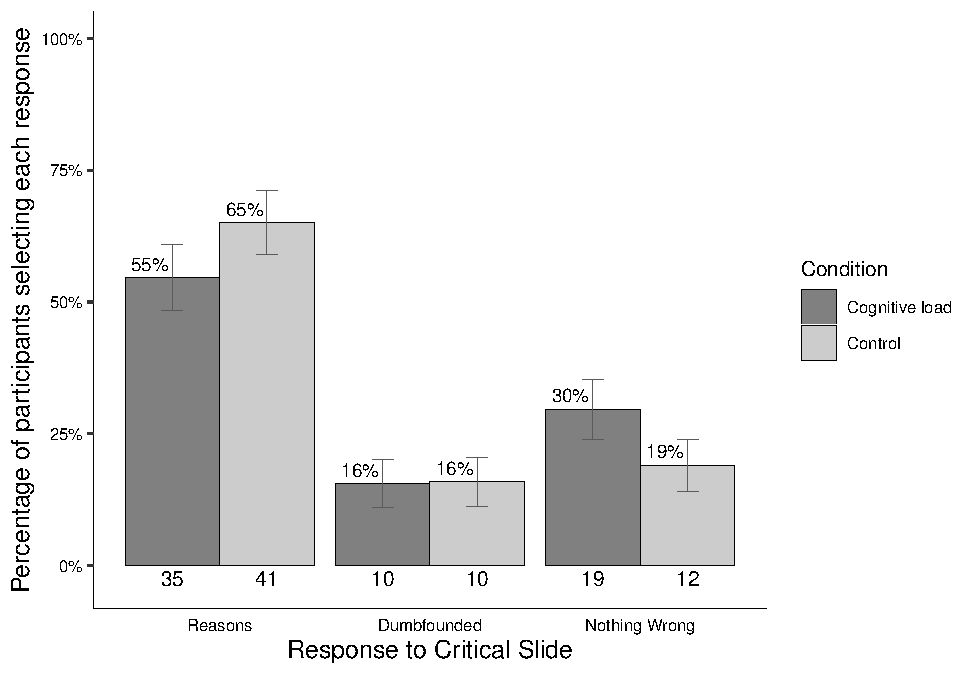
\includegraphics{Supplementary_files/figure-latex/ch5S4fig2criticalcondition-1} \caption{Study S4: Responses to critical slide for the cognitive load group (N = 64) and the control group (N = 61); (error bars represent standard error of the proportion)}\label{fig:ch5S4fig2criticalcondition}
\end{figure}

\begin{figure}[!h]
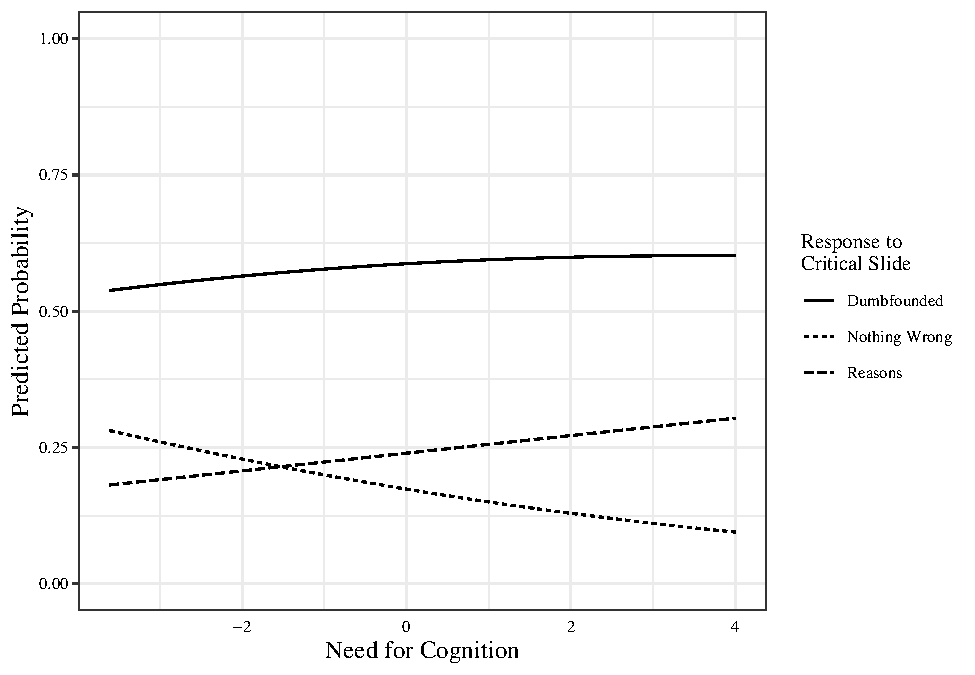
\includegraphics{Supplementary_files/figure-latex/ggplotlogit4-1} \caption{Study S4: Probability of selecting each response to the critical slide depending on Need for Cognition}\label{fig:ggplotlogit4}
\end{figure}

Ninety five participants (76.61\%) rated the behavior of Julie and Mark as wrong initially, and eighty nine participants (71.77\%) rated the behavior as wrong at the end of the task. Initial ratings (\emph{M} = 2.12, \emph{SD} = 1.63) were significantly more severe than revised ratings (\emph{M} = 2.34, \emph{SD} = 1.80), \emph{t}(123) = -3.14, \emph{p} = .002; \emph{d} = 0.28. Inspection of the binned judgments revealed that thirteen participants changed the valence of their judgments, and all but two of these involved one judgment that was neutral (see Table~\ref{tab:tabS4change}).

\begin{table}[tbp]

\begin{center}
\begin{threeparttable}

\caption{\label{tab:tabS4change}Study S4 – Changes in Jugment}

\begin{tabular}{ccc}
\toprule
Initial Judgment & \multicolumn{1}{c}{Revised Judgment} & \multicolumn{1}{c}{Total Changed}\\
\midrule
neutral & right & 4\\
right & neutral & 1\\
right & wrong & 1\\
wrong & neutral & 6\\
wrong & right & 1\\
\bottomrule
\end{tabular}

\end{threeparttable}
\end{center}

\end{table}

\begin{table}[tbp]

\begin{center}
\begin{threeparttable}

\caption{\label{tab:tabS4tab1dumb1all}Study S4 – Response to the critical slide depending on cognitive load/engagement}

\begin{tabular}{llccc}
\toprule
 & \multicolumn{2}{c}{Cognitive Load} & \multicolumn{2}{c}{Control} \\
\cmidrule(r){2-3} \cmidrule(r){4-5}
 & \multicolumn{1}{c}{N} & \multicolumn{1}{c}{\%} & \multicolumn{1}{c}{N} & \multicolumn{1}{c}{\%}\\
\midrule
It's wrong and I can provide a valid reason. & 34 & 54\% & 39 & 64\%\\
It's wrong but I can't think of a reason. & 10 & 16\% & 10 & 16\%\\
There is nothing wrong. & 19 & 30\% & 12 & 20\%\\
\bottomrule
\end{tabular}

\end{threeparttable}
\end{center}

\end{table}

Investigation of the responses to the manipulation check questions revealed no difference in the number of correct answers to these questions between the cognitive load group and the control group \emph{t}(121.92) = 0.50, \emph{p} = .618; \emph{d} = 0.09. There was also no difference in time taken to read the vignette between the groups \emph{t}(62.41) = 1.62, \emph{p} = .111; \emph{d} = 0.29.

\begin{table}[tbp]

\begin{center}
\begin{threeparttable}

\caption{\label{tab:S4tab1dumb}Study S4 – Observed counts, expected counts, and standardised residuals for each response to the critical slide depending on cognitive load}

\begin{tabular}{llcc}
\toprule
 & \multicolumn{1}{c}{} & \multicolumn{1}{c}{Cognitive Load} & \multicolumn{1}{c}{Control}\\
\midrule
Observed count & Reasons & 34.00 & 39.00\\
 & Dumbfounded & 10.00 & 10.00\\
 & Nothing Wrong & 19.00 & 12.00\\
Expected count & Reasons & 37.09 & 35.91\\
 & Dumbfounded & 10.16 & 9.84\\
 & Nothing Wrong & 15.75 & 15.25\\
Standardised residuals & Reasons & -1.13 & 1.13\\
 & Dumbfounded & -0.08 & 0.08\\
 & Nothing Wrong & 1.35 & -1.35\\
\bottomrule
\addlinespace
\end{tabular}

\begin{tablenotes}[para]
\normalsize{\textit{Note.} * = sig. at \emph{p} < .05; ** = sig. at \emph{p} < .001}
\end{tablenotes}

\end{threeparttable}
\end{center}

\end{table}

On the critical slide, twenty participants (16.13\%) selected ``It's wrong but I can't think of a reason''. Seventy three participants (58.87\%) selected ``It's wrong and I can provide a valid reason''; and thirty one participants (25\%) selected ``There is nothing wrong''.

A chi-squared test for independence revealed no significant association between experimental condition and response to the critical slide, \(\chi\)\textsuperscript{2}(2, \emph{N} = 124) = 1.89, \emph{p} = .388, \emph{V} = 0.12, the observed power was 0.22. The responses to the critical slide for the experimental group (\emph{N} = 63) and the control group (\emph{N} = 61) are displayed in Figure~\ref{fig:ch5S4fig2criticalcondition} and Table~\ref{tab:tabS4tab1dumb1all}. The observed counts, expected counts and standardised residuals are displayed in Table~\ref{tab:S4tab1dumb}.

A multinomial logistic regression revealed no statistically significant association between Need for Cognition and response to the critical slide, \(\chi\)\textsuperscript{2}(2, \emph{N} = 124) = 1.5, \emph{p} = .472, the observed power was 0.18 (see Figure~\ref{fig:ggplotlogit4} for relative probabilities of selecting each response depending on Need for Cognition).

\newpage

\hypertarget{study-s5-number-letter-task-college-sample}{%
\section{Study S5: Number-Letter Task (College Sample)}\label{study-s5-number-letter-task-college-sample}}

Given the inconclusive results across studies 1-4, Study S5 was to an attempt at a direct replication of Study S1, using a larger sample.

\hypertarget{study-s5-method}{%
\subsection{Study S5: Method}\label{study-s5-method}}

\hypertarget{study-s5-participants-and-design}{%
\subsubsection{Study S5: Participants and Design}\label{study-s5-participants-and-design}}

Study S5 was a between subjects design. The dependent variable was response to the critical slide. The independent variable was cognitive load with two levels: present and absent. Need for Cognition (Cacioppo \& Petty, 1982; Petty et al., 1984) was included as a potential correlate and moderator variable.

A total sample of 204 participants (144 female, 59 male; \emph{M}\textsubscript{age} = 20.56, min = 18, max = 48, \emph{SD} = 3.86) took part. Participants in this sample were undergraduate students, postgraduate students, and alumni from Mary Immaculate College (MIC), and University of Limerick (UL). Participation was voluntary and participants were not reimbursed for their participation.

\hypertarget{study-s5-procedure-and-materials}{%
\subsubsection{Study S5: Procedure and Materials}\label{study-s5-procedure-and-materials}}

Data were collected using an online questionnaire. Data collection took place in a designated computer laboratory in MIC. The experimenter remained in the laboratory for the duration of the study. Participants were first presented with an information sheet and consent form.

There were two sections of the online survey: the moral judgement task, and the Need for Cognition scale. The order of presentation of these was randomised. At the beginning of the moral judgement task, participants in the experimental condition were presented with an eight digit number/letter string and asked to memorise the sequence. After 30 seconds, the experiment progressed to the next slide. Participants had the option to click ``ok'' and progress to the next slide after 15 seconds.

Participants were then presented with the ``Julie and Mark'' (\emph{Incest}) vignette (Haidt et al., 2000). Participants rated how right or wrong the behaviour of Julie and Mark was, and were given an opportunity to provide reasons for their judgement. Following this, participants were presented with a series of counter-arguments, which refuted commonly used justifications for rating the behaviour as ``wrong''. Dumbfounding was measured using the critical slide. Following the revised judgement participants were required to reproduce the number/letter string.

\hypertarget{study-s5-results}{%
\subsection{Study S5: Results}\label{study-s5-results}}

\begin{figure}[!h]
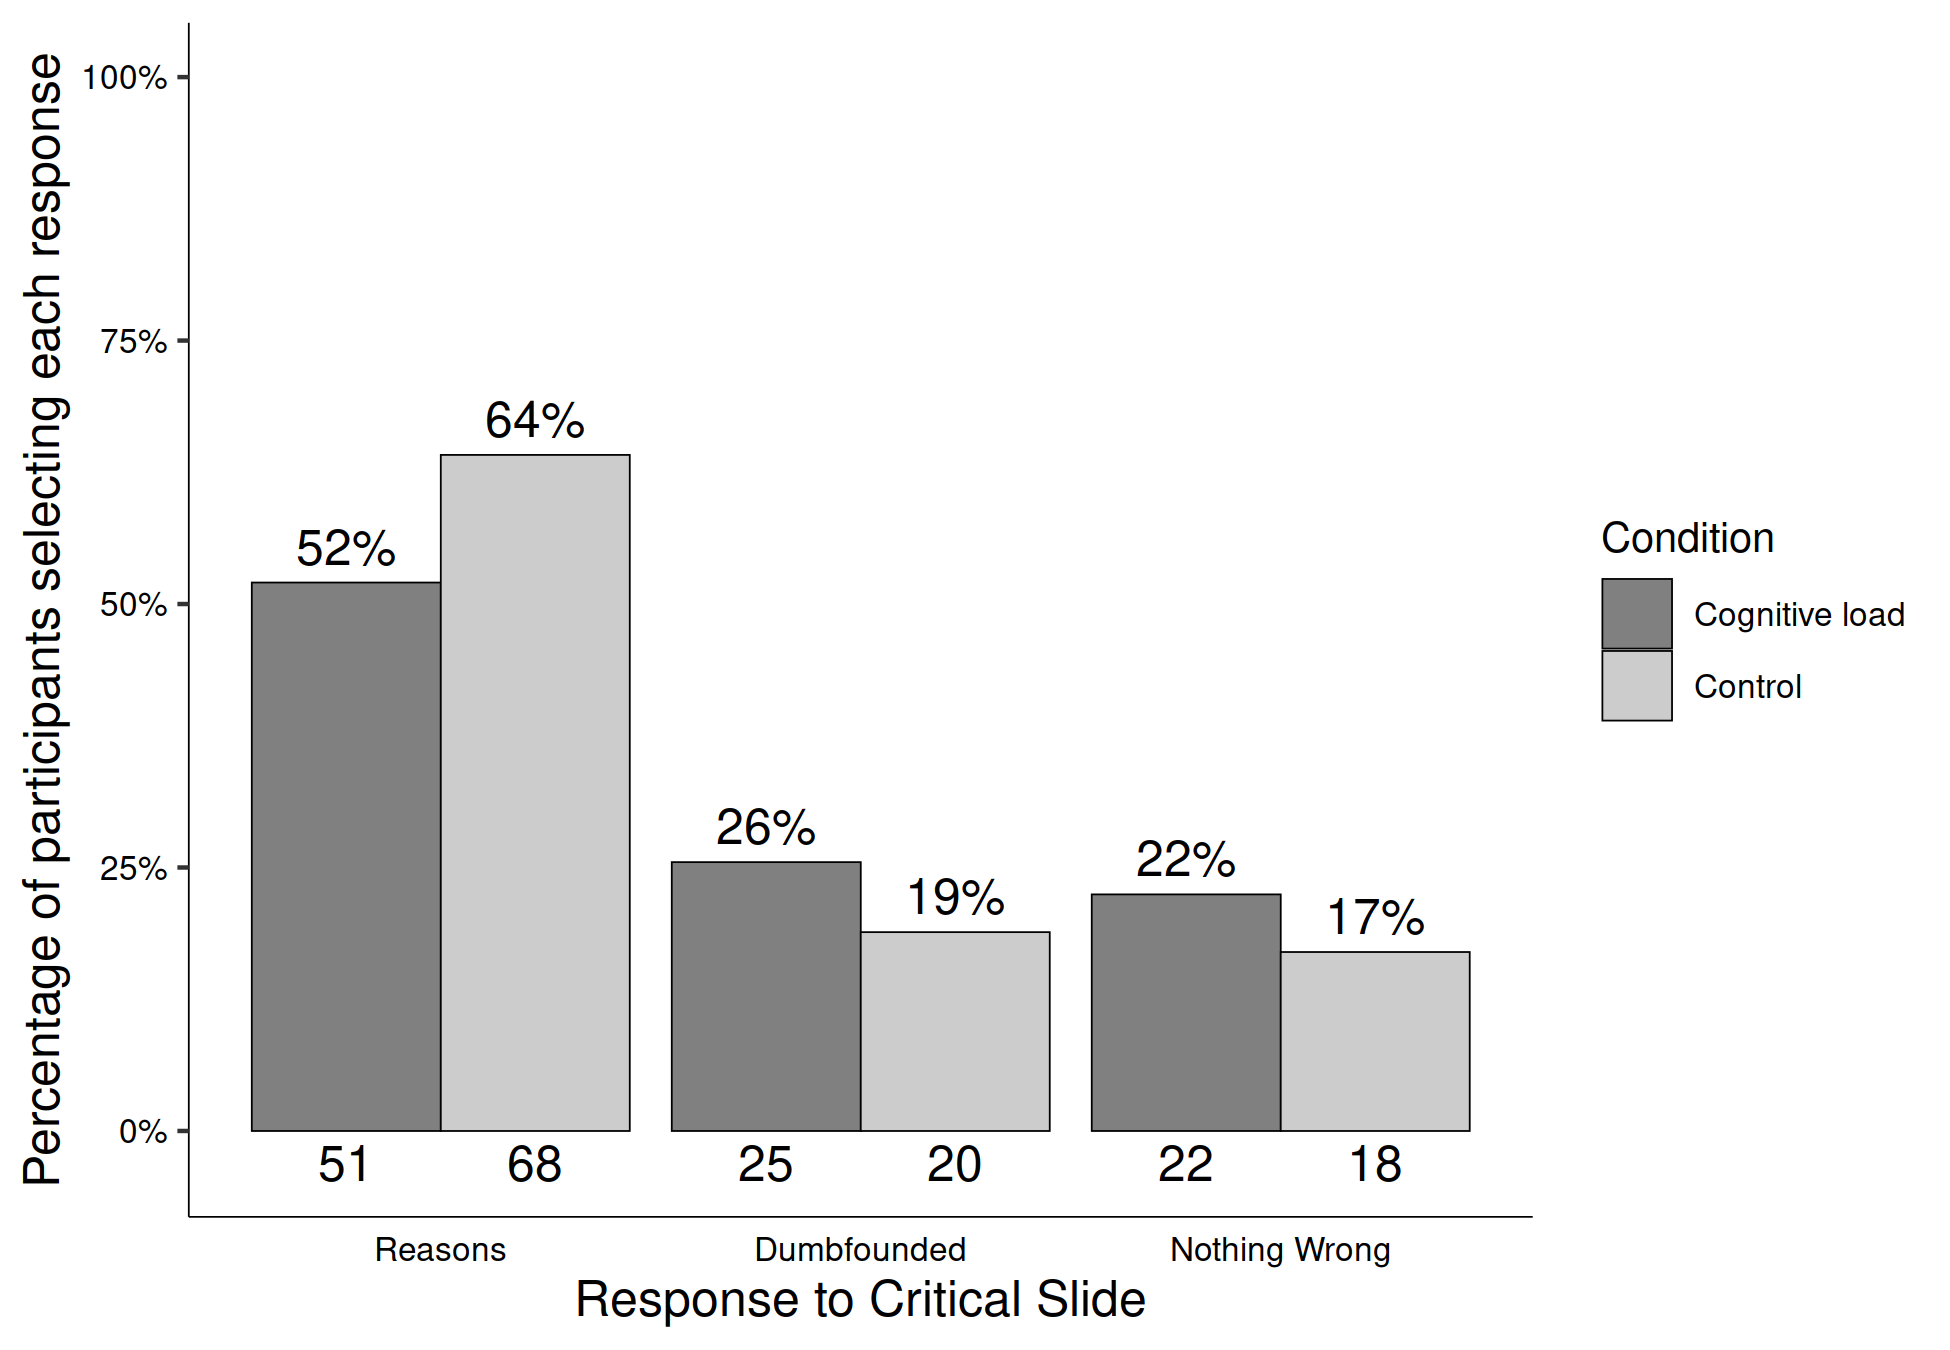
\includegraphics{Supplementary_files/figure-latex/ch5S5fig2criticalcondition-1} \caption{Study S5: Responses to critical slide and for the experimental group (N = 98) and the control group (N = 106); (error bars represent standard error of the proportion)}\label{fig:ch5S5fig2criticalcondition}
\end{figure}

\begin{figure}[!h]
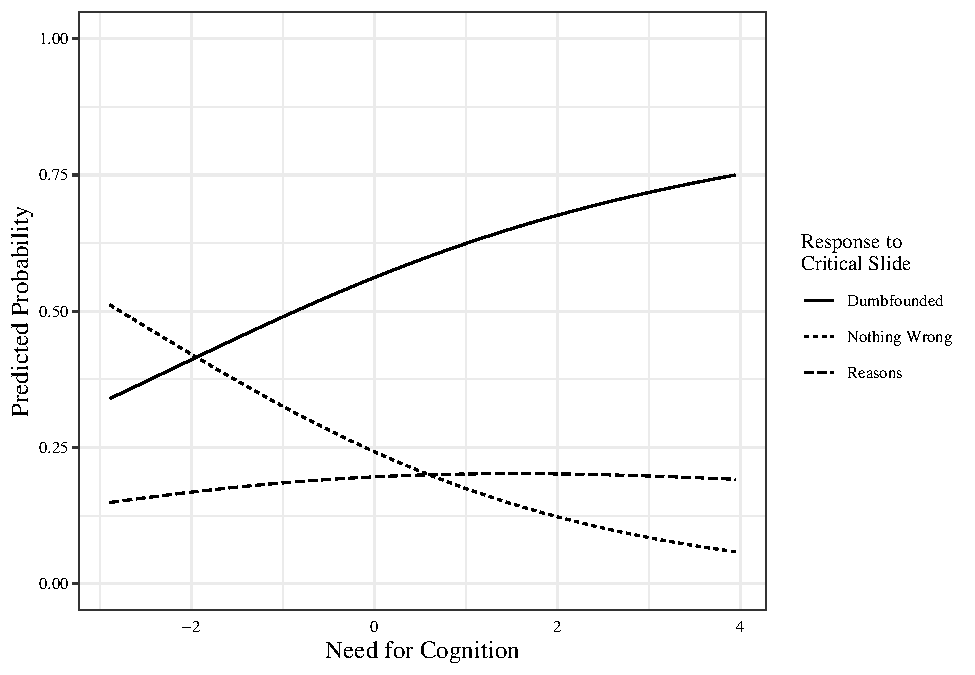
\includegraphics{Supplementary_files/figure-latex/ggplotlogit5-1} \caption{Study S5: Probability of selecting each response to the critical slide depending on Need for Cognition}\label{fig:ggplotlogit5}
\end{figure}

One hundred and sixty-five participants (80.88\%) rated the behavior of Julie and Mark as wrong initially, and one hundred fifty nine participants (77.94\%) rated the behavior as wrong at the end of the task. Initial ratings (\emph{M} = 2.01, \emph{SD} = 1.82) were significantly more severe than revised ratings (\emph{M} = 2.20, \emph{SD} = 1.77), \emph{t}(203) = -3.42, \emph{p} \textless{} .001; \emph{d} = 0.24. Inspection of the binned judgments revealed that eleven participants changed the valence of their judgments, and all but two of these involved one judgment that was neutral (see Table~\ref{tab:tabS5change}).

\begin{table}[tbp]

\begin{center}
\begin{threeparttable}

\caption{\label{tab:tabS5change}Study S5 – Changes in Jugment}

\begin{tabular}{ccc}
\toprule
Initial Judgment & \multicolumn{1}{c}{Revised Judgment} & \multicolumn{1}{c}{Total Changed}\\
\midrule
neutral & right & 1\\
right & neutral & 2\\
right & wrong & 1\\
wrong & neutral & 6\\
wrong & right & 1\\
\bottomrule
\end{tabular}

\end{threeparttable}
\end{center}

\end{table}

\begin{table}[tbp]

\begin{center}
\begin{threeparttable}

\caption{\label{tab:tabS5tab1dumb1all}Study S5 – Response to the critical slide depending on cognitive load/engagement}

\begin{tabular}{llccc}
\toprule
 & \multicolumn{2}{c}{Cognitive Load} & \multicolumn{2}{c}{Control} \\
\cmidrule(r){2-3} \cmidrule(r){4-5}
 & \multicolumn{1}{c}{N} & \multicolumn{1}{c}{\%} & \multicolumn{1}{c}{N} & \multicolumn{1}{c}{\%}\\
\midrule
It's wrong and I can provide a valid reason. & 51 & 52\% & 68 & 64\%\\
It's wrong but I can't think of a reason. & 25 & 26\% & 20 & 19\%\\
There is nothing wrong. & 22 & 22\% & 18 & 17\%\\
\bottomrule
\end{tabular}

\end{threeparttable}
\end{center}

\end{table}

\begin{table}[tbp]

\begin{center}
\begin{threeparttable}

\caption{\label{tab:S5tab1dumb}Study S5 – Observed counts, expected counts, and standardised residuals for each response to the critical slide depending on cognitive load}

\begin{tabular}{llcc}
\toprule
 & \multicolumn{1}{c}{} & \multicolumn{1}{c}{Cognitive Load} & \multicolumn{1}{c}{Control}\\
\midrule
Observed count & Reasons & 51.00 & 68.00\\
 & Dumbfounded & 25.00 & 20.00\\
 & Nothing Wrong & 22.00 & 18.00\\
Expected count & Reasons & 57.17 & 61.83\\
 & Dumbfounded & 21.62 & 23.38\\
 & Nothing Wrong & 19.22 & 20.78\\
Standardised residuals & Reasons & -1.75 & 1.75\\
 & Dumbfounded & 1.14 & -1.14\\
 & Nothing Wrong & 0.98 & -0.98\\
\bottomrule
\addlinespace
\end{tabular}

\begin{tablenotes}[para]
\normalsize{\textit{Note.} * = sig. at \emph{p} < .05; ** = sig. at \emph{p} < .001}
\end{tablenotes}

\end{threeparttable}
\end{center}

\end{table}

Next we examined responses to the critical slide. Forty five participants (22.06\%) selected ``It's wrong but I can't think of a reason''. one hundred Nineteen participants (58.33\%) selected ``It's wrong and I can provide a valid reason''; and forty participants (19.61\%) selected ``There is nothing wrong''.

Initial check of responses to the memory task revealed that 42 participants (42.86\%) successfully remembered the sequence of numbers and letters. Responses to the manipulation check question revealed that 22 participants (22.45\%) found the memory task easy. Of these, 20 participants both found the task easy and got the answer right. All participants correctly remembered at least two digits suggesting engagement with the manipulation.

The cognitive load manipulation took place before the presenting of the vignette describing the behaviour to be judged. This allowed for the possibility that participants under cognitive load may not have engaged fully with the vignette when compared to the control group. An independent samples t-test revealed no significant difference in initial rating in the cognitive load group, (\emph{M} = 2.15, \emph{SD} = 1.97), and the control group, (\emph{M} = 2.05, \emph{SD} = 1.66), \emph{t}(191.10) = 1.04 , \emph{p} = 0.30; \emph{d} = 0.15. An independent samples t-test revealed no significant difference in initial confidence in the cognitive load group, (\emph{M} = 5.51, \emph{SD} = 1.55), and the control group, (\emph{M} = 5.83, \emph{SD} = 1.49), \emph{t}(199.05) = -1.50 , \emph{p} = 0.14; \emph{d} = 0.21. In view of this, it was concluded that both groups engaged equally with the task.

To test our hypothesis we conducted a chi-squared test for independence that revealed no significant association between experimental condition and response to the critical slide, \(\chi\)\textsuperscript{2}(2, \emph{N} = 204) = 3.08, \emph{p} = .215, \emph{V} = 0.12, the observed power was 0.33. The predicted relationship between cognitive load and dumbfounded responding was not observed in Study S5. The responses to the critical slide for the experimental group (\emph{N} = 98) and the control group (\emph{N} = 106) are displayed in Figure~\ref{fig:ch5S5fig2criticalcondition} and Table~\ref{tab:tabS5tab1dumb1all}. The observed counts, expected counts and standardised residuals are displayed in Table~\ref{tab:S5tab1dumb}.

A multinomial logistic regression revealed no significant association between Need for Cognition and response to the critical slide, \(\chi\)\textsuperscript{2}(2, \emph{N} = 204) = 5.83, \emph{p} = .054, The observed
power was 0.57.

\newpage

~

\hypertarget{supplementary-tables}{%
\section{Supplementary Tables}\label{supplementary-tables}}

\newpage

~

\begin{table}[tbp]

\begin{center}
\begin{threeparttable}

\caption{\label{tab:tabS6change}Changes in Jugment (full sample)}

\begin{tabular}{ccc}
\toprule
Initial Judgment & \multicolumn{1}{c}{Revised Judgment} & \multicolumn{1}{c}{Total Changed}\\
\midrule
neutral & right & 8\\
neutral & wrong & 19\\
right & neutral & 10\\
right & wrong & 61\\
wrong & neutral & 29\\
wrong & right & 73\\
\bottomrule
\end{tabular}

\end{threeparttable}
\end{center}

\end{table}

\begin{table}[tbp]

\begin{center}
\begin{threeparttable}

\caption{\label{tab:tabS6changeeachscenario}Changes in Jugment for each Scenario}

\begin{tabular}{lccc}
\toprule
Scenario & \multicolumn{1}{c}{Initial Judgment} & \multicolumn{1}{c}{Revised Judgment} & \multicolumn{1}{c}{Total Changed}\\
\midrule
Julie and Mark & neutral & right & 1\\
 & neutral & wrong & 4\\
 & right & wrong & 6\\
 & wrong & neutral & 9\\
 & wrong & right & 8\\
Jennifer & neutral & right & 1\\
 & neutral & wrong & 3\\
 & right & neutral & 2\\
 & right & wrong & 10\\
 & wrong & neutral & 2\\
 & wrong & right & 11\\
Trolley & neutral & right & 4\\
 & neutral & wrong & 7\\
 & right & neutral & 4\\
 & right & wrong & 18\\
 & wrong & neutral & 14\\
 & wrong & right & 26\\
Heinz & neutral & right & 2\\
 & neutral & wrong & 5\\
 & right & neutral & 4\\
 & right & wrong & 27\\
 & wrong & neutral & 4\\
 & wrong & right & 28\\
\bottomrule
\end{tabular}

\end{threeparttable}
\end{center}

\end{table}

\begin{table}[tbp]

\begin{center}
\begin{threeparttable}

\caption{\label{tab:tabS6tab1dumb1all}Response to the critical slide depending on cognitive load (full sample)}

\begin{tabular}{lcccc}
\toprule
 & \multicolumn{2}{c}{Cognitive Load} & \multicolumn{2}{c}{Control} \\
\cmidrule(r){2-3} \cmidrule(r){4-5}
 & \multicolumn{1}{c}{N} & \multicolumn{1}{c}{\%} & \multicolumn{1}{c}{N} & \multicolumn{1}{c}{\%}\\
\midrule
It's wrong and I can provide a valid reason. & 458 & 55\% & 574 & 67\%\\
It's wrong but I can't think of a reason. & 245 & 30\% & 172 & 20\%\\
There is nothing wrong. & 123 & 15\% & 114 & 13\%\\
\bottomrule
\end{tabular}

\end{threeparttable}
\end{center}

\end{table}

\begin{table}[tbp]

\begin{center}
\begin{threeparttable}

\caption{\label{tab:tabS6tab1dumb1allIncest}Response to the critical slide depending on cognitive load, for each scenario}

\begin{tabular}{llcccc}
\toprule
 &  & \multicolumn{2}{c}{Cognitive Load} & \multicolumn{2}{c}{Control} \\
\cmidrule(r){3-4} \cmidrule(r){5-6}
Scenario & \multicolumn{1}{c}{Response} & \multicolumn{1}{c}{N} & \multicolumn{1}{c}{\%} & \multicolumn{1}{c}{N} & \multicolumn{1}{c}{\%}\\
\midrule
Julie and Mark & Reasons & 106 & 54\% & 123 & 57\%\\
 & Dumbfounded & 51 & 26\% & 51 & 24\%\\
 & Nothing Wrong & 40 & 20\% & 41 & 19\%\\
Jennifer & Reasons & 142 & 65\% & 173 & 81\%\\
 & Dumbfounded & 67 & 31\% & 30 & 14\%\\
 & Nothing Wrong & 9 & 4\% & 11 & 5\%\\
Trolley & Reasons & 97 & 47\% & 135 & 62\%\\
 & Dumbfounded & 72 & 35\% & 55 & 25\%\\
 & Nothing Wrong & 39 & 19\% & 26 & 12\%\\
Heinz & Reasons & 113 & 56\% & 143 & 67\%\\
 & Dumbfounded & 55 & 27\% & 36 & 17\%\\
 & Nothing Wrong & 35 & 17\% & 36 & 17\%\\
\bottomrule
\end{tabular}

\end{threeparttable}
\end{center}

\end{table}

\begin{table}[tbp]

\begin{center}
\begin{threeparttable}

\caption{\label{tab:tabS6tab1dumbIncest}Observed counts, expected counts, and standardised residuals for each response to the critical slide depending on cognitive load (Julie and Mark)}

\begin{tabular}{llcc}
\toprule
 & \multicolumn{1}{c}{} & \multicolumn{1}{c}{Cognitive Load} & \multicolumn{1}{c}{Control}\\
\midrule
Observed count & Reasons & 106 & 123\\
 & Dumbfounded & 51 & 51\\
 & Nothing Wrong & 40 & 41\\
Expected count & Reasons & 109.5 & 119.5\\
 & Dumbfounded & 48.77 & 53.23\\
 & Nothing Wrong & 38.73 & 42.27\\
Standardised residuals & Reasons & -0.69 & 0.69\\
 & Dumbfounded & 0.51 & -0.51\\
 & Nothing Wrong & 0.32 & -0.32\\
\bottomrule
\addlinespace
\end{tabular}

\begin{tablenotes}[para]
\normalsize{\textit{Note.} * = sig. at \emph{p} < .05; ** = sig. at \emph{p} < .001}
\end{tablenotes}

\end{threeparttable}
\end{center}

\end{table}

\begin{table}[tbp]

\begin{center}
\begin{threeparttable}

\caption{\label{tab:tabS6tab1dumbJennifer}Observed counts, expected counts, and standardised residuals for each response to the critical slide depending on cognitive load (Jennifer)}

\begin{tabular}{llcc}
\toprule
 & \multicolumn{1}{c}{} & \multicolumn{1}{c}{Cognitive Load} & \multicolumn{1}{c}{Control}\\
\midrule
Observed count & Reasons & 142 & 173\\
 & Dumbfounded & 67 & 30\\
 & Nothing Wrong & 9 & 11\\
Expected count & Reasons & 158.96 & 156.04\\
 & Dumbfounded & 48.95 & 48.05\\
 & Nothing Wrong & 10.09 & 9.91\\
Standardised residuals & Reasons & -3.67** & 3.67**\\
 & Dumbfounded & 4.16** & -4.16**\\
 & Nothing Wrong & -0.5 & 0.5\\
\bottomrule
\addlinespace
\end{tabular}

\begin{tablenotes}[para]
\normalsize{\textit{Note.} * = sig. at \emph{p} < .05; ** = sig. at \emph{p} < .001}
\end{tablenotes}

\end{threeparttable}
\end{center}

\end{table}

\begin{table}[tbp]

\begin{center}
\begin{threeparttable}

\caption{\label{tab:tabS6tab1dumbTrolley}Observed counts, expected counts, and standardised residuals for each response to the critical slide depending on cognitive load (Trolley)}

\begin{tabular}{llcc}
\toprule
 & \multicolumn{1}{c}{} & \multicolumn{1}{c}{Cognitive Load} & \multicolumn{1}{c}{Control}\\
\midrule
Observed count & Reasons & 97 & 135\\
 & Dumbfounded & 72 & 55\\
 & Nothing Wrong & 39 & 26\\
Expected count & Reasons & 113.81 & 118.19\\
 & Dumbfounded & 62.3 & 64.7\\
 & Nothing Wrong & 31.89 & 33.11\\
Standardised residuals & Reasons & -3.28* & 3.28*\\
 & Dumbfounded & 2.06* & -2.06*\\
 & Nothing Wrong & 1.92 & -1.92\\
\bottomrule
\addlinespace
\end{tabular}

\begin{tablenotes}[para]
\normalsize{\textit{Note.} * = sig. at \emph{p} < .05; ** = sig. at \emph{p} < .001}
\end{tablenotes}

\end{threeparttable}
\end{center}

\end{table}

\begin{table}[tbp]

\begin{center}
\begin{threeparttable}

\caption{\label{tab:tabS6tab1dumbHeinz}Observed counts, expected counts, and standardised residuals for each response to the critical slide depending on cognitive load (Heinz)}

\begin{tabular}{llcc}
\toprule
 & \multicolumn{1}{c}{} & \multicolumn{1}{c}{Cognitive Load} & \multicolumn{1}{c}{Control}\\
\midrule
Observed count & Reasons & 113 & 143\\
 & Dumbfounded & 55 & 36\\
 & Nothing Wrong & 35 & 36\\
Expected count & Reasons & 124.33 & 131.67\\
 & Dumbfounded & 44.19 & 46.81\\
 & Nothing Wrong & 34.48 & 36.52\\
Standardised residuals & Reasons & -2.27* & 2.27*\\
 & Dumbfounded & 2.56* & -2.56*\\
 & Nothing Wrong & 0.14 & -0.14\\
\bottomrule
\addlinespace
\end{tabular}

\begin{tablenotes}[para]
\normalsize{\textit{Note.} * = sig. at \emph{p} < .05; ** = sig. at \emph{p} < .001}
\end{tablenotes}

\end{threeparttable}
\end{center}

\end{table}

\begin{table}[tbp]

\begin{center}
\begin{threeparttable}

\caption{\label{tab:tabS6EngagementAndDumbfounding}Study 6 – Response to the critical slide depending on performance in cognitive load task}

\begin{tabular}{lcccc}
\toprule
 & \multicolumn{2}{c}{Correct} & \multicolumn{2}{c}{Incorrect} \\
\cmidrule(r){2-3} \cmidrule(r){4-5}
 & \multicolumn{1}{c}{N} & \multicolumn{1}{c}{\%} & \multicolumn{1}{c}{N} & \multicolumn{1}{c}{\%}\\
\midrule
It's wrong and I can provide a valid reason. & 203 & 53\% & 255 & 58\%\\
It's wrong but I can't think of a reason. & 127 & 33\% & 118 & 27\%\\
There is nothing wrong. & 53 & 14\% & 70 & 16\%\\
\bottomrule
\end{tabular}

\end{threeparttable}
\end{center}

\end{table}

\newpage

~

\newpage

~

\newpage

~

\newpage

~

\newpage

~

\newpage

~

\newpage

\hypertarget{references}{%
\section{References}\label{references}}

\setlength{\parindent}{-0.5in}
\setlength{\leftskip}{0.5in}
\setlength{\parskip}{8pt}

\hypertarget{refs}{}
\begin{CSLReferences}{1}{0}
\leavevmode\vadjust pre{\hypertarget{ref-amazonwebservicesinc._amazon_2016}{}}%
Amazon Web Services Inc. (2016). \emph{Amazon {Mechanical Turk}}.

\leavevmode\vadjust pre{\hypertarget{ref-cacioppo_need_1982}{}}%
Cacioppo, J. T., \& Petty, R. E. (1982). The need for cognition. \emph{Journal of Personality and Social Psychology}, \emph{42}(1), 116--131. \url{https://doi.org/10.1037/0022-3514.42.1.116}

\leavevmode\vadjust pre{\hypertarget{ref-deneys_when_2007}{}}%
De Neys, W., \& Schaeken, W. (2007). When people are more logical under cognitive load: {Dual} task impact on scalar implicature. \emph{Experimental Psychology}, \emph{54}(2), 128--133. \url{https://doi.org/10.1027/1618-3169.54.2.128}

\leavevmode\vadjust pre{\hypertarget{ref-evans_dualprocess_2013}{}}%
Evans, J. St. B. T., \& Stanovich, K. E. (2013). Dual-{Process Theories} of {Higher Cognition}: {Advancing} the {Debate}. \emph{Perspectives on Psychological Science}, \emph{8}(3), 223--241. \url{https://doi.org/10.1177/1745691612460685}

\leavevmode\vadjust pre{\hypertarget{ref-forsterlee_examination_1999}{}}%
Forsterlee, R., \& Ho, R. (1999). An {Examination} of the {Short} form of the {Need} for {Cognition Scale Applied} in an {Australian Sample}. \emph{Educational and Psychological Measurement}, \emph{59}(3), 471--480. \url{https://doi.org/10.1177/00131649921969983}

\leavevmode\vadjust pre{\hypertarget{ref-haidt_moral_2000}{}}%
Haidt, J., Björklund, F., \& Murphy, S. (2000). Moral dumbfounding: {When} intuition finds no reason. \emph{Unpublished Manuscript, University of Virginia}.

\leavevmode\vadjust pre{\hypertarget{ref-just_capacity_1992}{}}%
Just, M. A., \& Carpenter, P. A. (1992). A capacity theory of comprehension: {Individual} differences in working memory. \emph{Psychological Review}, \emph{99}(1), 122--149. \url{https://doi.org/10.1037/0033-295X.99.1.122}

\leavevmode\vadjust pre{\hypertarget{ref-mchugh_searching_2017a}{}}%
McHugh, C., McGann, M., Igou, E. R., \& Kinsella, E. L. (2017). Searching for {Moral Dumbfounding}: {Identifying Measurable Indicators} of {Moral Dumbfounding}. \emph{Collabra: Psychology}, \emph{3}(1), 1--24. \url{https://doi.org/10.1525/collabra.79}

\leavevmode\vadjust pre{\hypertarget{ref-petty_efficient_1984}{}}%
Petty, R. E., Cacioppo, J. T., \& Kao, C. F. (1984). The efficient assessment of need for cognition. \emph{Journal of Personality Assessment}, \emph{48}(3), 306--307.

\leavevmode\vadjust pre{\hypertarget{ref-petty_dispositional_1996}{}}%
Petty, R. E., Feinstein, J. A., Blair, W., \& Jarvis, G. (1996). Dispositional differences in cognitive motivation: {The} life and times of individuals varying in need for cognition. \emph{Psych. Bull}, 197--253.

\end{CSLReferences}


\end{document}
